% %%%%%%%%%%%%%%%%%%%%%%%%%%%%%%%%%%%%%%%%%%%%%%%%%%%%%%%%%%%%%%%%%%%%%%%%%%%%%%%% %
%
%	MODELO LaTeX PARA ELABORACAO DE TESES E DISSERTACOES 
%  ----------------------------------------------------
%
%	BASEADO NA CLASSE PPGMAp.cls (Classe base: report.cls)
%  ------------------------------------------------------
%
%
%	Creditos
%
%		Autor: Guilherme F. Fornel (guilherme.fornel@ufrgs.br)
%	
%		! Se encontrar bugs envie um e-mail relatando !
%
%
%	Pacotes nativos da classe PPGMAp.cls (nao precisam ser adicionados pelo usuario)
%		
%		inputenc (utf8 encoding)
%		fontenc  (T1 encoding)
%		babel    (default: brazil - english, portuguese, french, spanish,
%				    german, russian)
%		etoolbox
%		nomencl  (intoc option)
%		lipsum
%		atbegshi
%		calc
%
%
%	Sobre a compilacao
%
%		E recomendavel a utilizacao da biblioteca/compilador TeX Live 2016 FULL
%		(este modelo foi compilado para teste com a versao 2016.20170123-5)
%
%		Para a instalacao do TeX Live em so's derivados do linux Ubuntu utilizar
%
%			sudo apt-get install texlive-full 
%
%		# Compilando o modelo via terminal do linux:
%
%			Para a compilacao via terminal utilizar as seguintes linhas de 
%			comando:
%
%			pdflatex nome_do_arquivo_principal
%			bibtex nome_do_arquivo_principal   <opcional>
%			makeindex -s nomencl.ist -t nome_do_arquivo_principal.nlg -o nome_do_arquivo_principal.nls nome_do_arquivo_principal.nlo <para lista de simbolos>
%			pdflatex nome_do_arquivo_principal
%			pdflatex nome_do_arquivo_principal
%
%			No caso deste modelo:
%
%			pdflatex main
%			bibtex main   <opcional>
%			makeindex -s nomencl.ist -t main.nlg -o main.nls main.nlo <para lista de simbolos>
%			pdflatex main
%			pdflatex main		
%
%		# Utilizando a ide TeXstudio:
%
%			Usuarios do TeXstudio devem configurar a ide para gerar a lista de 
%			simbolos acessando
%		
% 			Opções -> Configurar TeXstudio -> Compilação -> Comandos do usuário
%					-> Adicionar
%
%			Deve ser adicionado o comando Make Nomenclature com
%
%			Nome do comando:  user0:Make Nomenclature
%			Linha de comando: makeindex -s nomencl.ist -t %.nlg -o %.nls %.nlo
%
%			Para a compilacao utilizar:
%
%			Ferramentas -> Comandos -> PDFLaTeX
%			Ferramentas -> Comandos -> BibteX              <opcional>
%			Ferramentas -> Usuario  -> Make Nomenclature   <para lista de simbolos>
%			Ferramentas -> Comandos -> PDFLaTeX
%			Ferramentas -> Comandos -> PDFLaTeX
%


% %%%%%%%%%%%%%%%%%%%%%%%%%%%%%%%%%%%%%%%%%%%%%%%%%%%%%%%%%%%%%%%%%%%%%%%%%%%%%%%% %
%
%	Opcoes da classe PPGMAp.cls
%
%		Por padrao a classe esta configurada para tese de doutorado com texto em 
%		portugues, folha A4, tamanho de fonte 12pt e configuracao de impressao em
%		ambos os lados da folha. Ao usuario, porem, estao disponiveis algumas opcoes 
%		de configuracao:
%
%		qualification : opcao para texto de qualificacao
%
%		masters : dissertacao de mestrado
%
%		english : texto em ingles
%
%		oneside : opcao para configuracao de impressao em apenas um lado da folha
%					 (ficha catalografica tambem)
%
%		print : opcao de versao final do texto para impressao em apenas um lado 
%				  da folha, com excessao da primeira pagina (folha de rosto e ficha
%				  catalografica). Para tal sao inseridas paginas em branco no 
%				  documento, e o usuario deve selecionar no aplicativo de
%				  impressao do sistema operacional a opcao IMPRIMIR EM AMBOS OS LADOS
%		
%		Demais opcoes da classe base report.cls NAO sao repassadas a classe PPGMAp.cls
%	

% \documentclass[print,masters]{./config/PPGMAp}
\documentclass[masters]{./config/PPGMAp}


% %%%%%%%%%%%%%%%%%%%%%%%%%%%%%%%%%%%%%%%%%%%%%%%%%%%%%%%%%%%%%%%%%%%%%%%%%%%%%%%% %
%
%	Informacoes para os elementos pre-textuais
%
%		Observacoes
%
%			Algumas informacoes sao opcionais, como \coadvisor e \memberd
%
%			Por padrao a data do documento e a data de compilacao e a data da defesa
%			e especificada com o comando \date
%
%			Nas infomacoes onde e possivel especificar o genero do individuo,
%		   a seguinte convencao e adotada: 'a','A','f' ou 'F' para feminino,  
%		   caso contrario masculino (neste caso os colchetes [] NAO precisam
%			ser escritos).
%
%		   (A especificacao da opcao 'o' neste modelo se da somente para exibir que
%			nao ha nenhum efeito sobre o genero, o genero masculino sendo adotado. 
%			Obviamente, no caso de texto em ingles a especificacao de genero tambem 
%			nao tem nenhum efeito)
%

%
% Titulo e data da defesa:
%
\title{Jogos Evolucionários em Redes Finitas com Jogadores Hiper-Racionais}
\date{abril}{2021}

%
% Linha de pesquisa:
%
\area{Sistemas Não-Lineares, Biomatemática}

%
% Palavras-chave:
%	{palavra-chave 1}{palavra-chave 2}{palavra-chave 3}{palavra-chave 4}
%
% " Keywords:
%	  {keyword 1}{keyword 2}{keyword 3}{keyword 4} "
%
\keywords{Teoria dos Jogos}{Racionalidade}{Jogos Evolucionários}{Grafos}

%
% Autor:
% 	[genero<opcional>]{nome}{sobrenome}
%
\author[o]{Rafael Jacobs}{Kehl}

%
% Orientador (e, se ha, co-orientador):
% 	[genero<opcional>]{tratamento}{nome}{sobrenome}
%
\advisor{Prof. Dr.}{Jean Carlo Pech de}{Moraes}
%\coadvisor[a]{Profa. Dra.}{Nome}{Sobrenome}

%
% Membros da banca:
% 	{tratamento}{nome}{sobrenome}
%
\membera{Profa. Dra.}{Chiara}{Mocenni}{Università degli Studi di Siena}
\memberb{Prof. Dr.}{Marcelo}{De Carvalho Griebeler}{PPGE - UFRGS}
\memberc{Prof. Dr.}{Matheus}{Correia dos Santos}{PPGMAp - UFRGS}

%
% Se ha um quarto membro na banca:
%
%\memberd{Prof. Dr.}{Nome}{Sobrenome}{Instituição D}

%
% Coordenador(a) do PPGMAp:
% 	[genero<opcional>]{tratamento}{primeiro nome}{ultimo nome}
%
\PPGMApcoord{Prof. Dr.}{Lucas da Silva}{Oliveira}


% %%%%%%%%%%%%%%%%%%%%%%%%%%%%%%%%%%%%%%%%%%%%%%%%%%%%%%%%%%%%%%%%%%%%%%%%%%%%%%%% %
%
%	Pacotes utilizados, opcoes e comandos definidos pelo usuario
%
%
% \usepackage{mypreamble}
% \usepackage{mypackages}
% \usepackage{mycommands}
% ...
%

\usepackage{./config/pack-and-cmd} % preâmbulo em outro arquivo!

% Meus pacotes
\usepackage{tabularx}
\usepackage{multirow}
\usepackage{placeins}
%\usepackage{hyperref}
\usepackage{url}

% Meus newcommand
\newcommand{\G}[0]{\mathcal{G}}
\newcommand{\V}[0]{\mathcal{V}}
\newcommand{\Rc}[0]{\mathcal{R}}
\newcommand{\BS}[1]{\boldsymbol{#1}}
\newtheorem{theorem}{Teorema}[section]
\newtheorem{lemma}[theorem]{Lema}
\theoremstyle{definition}
\newtheorem{definition}{Definição}[section]
\newcommand{\pdv}[3][]{\frac{\partial^{#1}#2}{\partial {#3}^{#1}}}


% %%%%%%%%%%%%%%%%%%%%%%%%%%%%%%%%%%%%%%%%%%%%%%%%%%%%%%%%%%%%%%%%%%%%%%%%%%%%%%%% %
%
%	Definicoes de nomenclaturas (siglas, simbolos e constantes fisicas)
%
%		A classe PPGMAp.cls utiliza o pacote nomenclature.sty para a criacao da
%		lista de siglas e simbolos. Isto possibilita ao usuario inserir 
%		facilmente Siglas, Simbolos e Constantes Fisicas respectivamente com os
%		comandos \Abbrev, \Symbol e \PConst definidos na classe PPGMAp.cls
%
%		Apesar de neste modelo os simbolos estarem especificados no preambulo
%		estes comandos (a principio) podem ser especificados tambem em quaisquer 
%     lugares dentro do ambiente de documento.	
%
%		Dupla insercao de simbolos (a principio) e desconsiderada.
%
%		O arquivo .nls necessario para a lista e gerado com o comando
%
%		makeindex main.nlo -s nomencl.ist -o main.nls
%

\Abbrev{PVI}{Problema de Valor Inicial}%

\Symbol{$E$}{Espaço métrico.}%

\Symbol{$d(x,y)$}{Distância entre os pontos $x$ e $y$ em um espaço métrico. A métrica do espaço.}%

\Symbol{$T$}{Transformação linear.}%

\Symbol{$C$}{Curva lisa.}%

\Symbol{$\nabla F$}{Vetor gradiente da função $F$.}%

\Symbol{$K$}{Conjunto compacto.}%

\Symbol{$\Omega$}{Produto cartesiano de um subconjunto aberto de $\R$ com um espaço métrico}

\Symbol{$\R$}{Conjunto dos números reais.}

\Symbol{$\partial\Omega$}{Fronteira do conjunto $\Omega$.}

\Symbol{$\V$}{Conjunto de jogadores. Conjunto de jogadores vértice.}%

\Symbol{$S_i$}{Conjunto de estratégias puras do jogador $i$.}%

\Symbol{$\BS{S}$}{Espaço de estratégias do jogo.}%

\Symbol{$u_i(\BS{s})$}{Função de pagamentos clássica do jogador $i$ para o perfil de estratégias do jogo $\BS{s}$.}%

\Symbol{$\Delta_M$}{Conjunto de estratégias mistas para um jogador com $M$ estratégias.}%

\Symbol{$\Delta$}{Espaço de estratégias mistas do jogo.}%

\Symbol{$\BS{X}$}{Perfil de estratégias do jogo evolucionário.}

\Symbol{$\BS{x}$}{Distribuição de estratégias de uma população.}

\Symbol{$B_v$}{Matriz de pagamentos do jogador $v$. Somente $B$ se for a única matriz de pagamentos do jogo.}

\Symbol{$\BS{e_i}$}{Vetor unitário cuja $i$-ésima entrada é igual a $1$.}

\Symbol{$\pi_s(\BS{x})$}{Aptidão do fenótipo $\BS{s}\in\BS{S}$ em uma população com distribuição $\BS{x}$.}

\Symbol{$\phi(\BS{x})$}{Aptidão média de uma população com distribuição $\BS{x}$.}

\Symbol{$\pi_{v,s}(\BS{X})$}{Pagamento de $v$ ao usar a estratégia $s$ em um jogo com perfil de estratégias $\BS{X}$. Também $\pi^\G_{v,s}(\BS{X})$ e $\pi^\mathcal{H}_{v,s}(\BS{X})$ para jogos em grafos e hiper-racionais, respectivamente.}

\Symbol{$\phi_v(\BS{X})$}{Pagamento médio de $v$ em um jogo com perfil de estratégias $\BS{X}$. Também $\phi^\G_v(\BS{X})$ e $\phi^\mathcal{H}_v(\BS{X})$ para jogos em grafos e hiper-racionais, respectivamente.}

\Symbol{$\Rc$}{Matriz de preferências de um jogo com jogadores hiper-racionais.}

\Symbol{$k_v(\BS{X})$}{Jogador vizinhança do jogador $v$ no jogo com perfil de estratégias $\BS{X}$.}

\Symbol{$\G$}{Grafo ou rede de conexões.}

\Symbol{$A$}{Matriz de adjacências que descreve o grafo $\G$.}

\Symbol{$\preceq$}{Relação qualquer. Neste contexto, indica preferência.}

\Symbol{$\gamma_{v,s}(t)$}{Parte social da equação de replicação hiper-racional.}

\Symbol{$\psi_{v,s}(t)$}{Parte pessoal da equação de replicação hiper-racional.}

\Symbol{$d_v$}{Grau do vértice $v$. Também $d_{v,r}$ como o grau de preferências de $v$.}

% %%%%%%%%%%%%%%%%%%%%%%%%%%%%%%%%%%%%%%%%%%%%%%%%%%%%%%%%%%%%%%%%%%%%%%%%%%%%%%%% %
%
%	Ambiente de documento
%
%		Sao declarados, alem de comandos para impressao de elementos obrigatorios
%		no texto, alguns ambientes de insercao (obrigatorios ou nao) nativos
%		da classe report.cls ou definidos na classe PPGMAp.cls.
%
%		Sao indicados dois sistemas de insercao de referencias bibliograficas,
%		o nativo e o com Bibtex.
%
%		A forma adotada para a declaracao dos elementos no ambiente documento visa 
%		dar alguma liberdade de modificacao do texto ao usuario.
%

\begin{document}

% !TeX root = ../thesis.tex

% defining tikz decoration -dot-:
\tikzset{
    -dot-/.style={
        decoration={
            markings,
            mark=at position #1 with {
                \fill circle (1.5pt);
            }
        },
        postaction={decorate}
    }
}

% defining tikz decoration ->:
\tikzset{
    ->-/.style={
        decoration={
            markings,
            mark=at position #1 with {
                \arrow{>}
            }
        },
        postaction={decorate}
    }
}

%
%	Elementos pre-textuais:
%
\frontmatter % formatacao do estilo dos elementos pre-textuais

%	Impressao da folha de rosto:
	\coversheet

%	Impressao da ficha catalografica:
	\catalogsheet

%	Impressao da folha de aprovacao:
	\approvalsheet

%	Epigrafe:
%		Entre colchetes e especificada a porcentagem da largura da pagina destinada
%		a epigrafe (padrao 0.5)
	\begin{epigraph}[0.5]
		{``Todos animais são iguais, mas alguns animais são mais iguais que os outros''} \\ \vspace{.25cm}
        \hfill -- George Orwell
	\end{epigraph}

%	Agradecimentos <ambiente>:
	\begin{acknowledgments}
		Aos meus pais que me incentivaram e ensinaram a importância do estudo. Sem o apoio, paciência, incentivo e exemplo deles nada disso seria possível. Também ao meu irmão, que contribuiu com este trabalho no tratamento das imagens e gráficos.
		
		Ao meu orientador, Jean, que direcionou a pesquisa e proveu muitos dos recursos necessários para a realização deste trabalho, além de sempre estar aberto para tirar minhas dúvidas e debater sobre o trabalho.  
		
		À minha namorada, que esteve do meu lado durante todo o mestrado me dando apoio e atenção. Tua presença sempre me acalma e me dá a clareza necessária para seguir em frente.
	\end{acknowledgments}

%	Impressao do sumario:
	\tableofcontents

%	Impressao da lista de figuras:
	\listoffigures

%	Impressao da lista de tabelas:
	\listoftables

%	Impressao da lista de siglas e simbolos:
%		Entre colchetes e especificado um parametro de comprimento do campo de
%		simbolo (padrao 2).
%	\printnomenclature[6]
	\printnomenclature

%	Resumo <ambiente>:
	\begin{resumo}
		Este trabalho propõe um novo modelo matemático para dinâmicas evolucionárias em redes finitas. Esse modelo estende a equação de replicação em redes finitas para jogadores hiper-racionais, que são capazes de considerar o benefício ou prejuízo dos demais jogadores na escolha de sua estratégia. Este processo é feito através da introdução de um novo parâmetro chamado matriz de preferências, que traz informações sobre a importância que um jogador dá para o benefício ou prejuízo de um outro jogador. A rede é modelada através de um grafo onde cada vértice do grafo representa uma subpopulação de replicadores hiper-racionais com mesma preferência que, a cada instante, interage com uma subpopulação vizinha e recebe um pagamento de acordo com suas preferências por si e por seus vizinhos. A equação obtida não depende de hipóteses sobre as matrizes de pagamento, topologia do grafo ou preferências dos jogadores. Os equilíbrios de Nash e o comportamento dos agentes hiper-racionais em diferentes jogos e grafos são discutidos. Também é feita uma comparação entre jogadores racionais e hiper-racionais para alguns jogos e grafos.
		
		\noindent \textbf{Palavras-chave:} Sistemas Não-Lineares; Biomatemática; Jogos Evolucionários.
	\end{resumo}

%	Abstract <ambiente>:
	\begin{abstract}
	    This work proposes a new mathematical model for evolutionary dynamics in finite networks. This model extends the replicator equation on networks to hyper-rational players, which considers the profit or the loss of others when choosing their strategy. This is made by adding a new parameter called matrix of preferences, which holds information on how much a player values the profit or the loss of another player. The network is represented by a graph where each vertex is interpreted as a subpopulation of hyper-rational replicators with the same preferences engaged at each time instant in 2-player games with a neighboring subpopulation, receiving a payoff according to their preferences. The obtained equation does not depends on any hypothesis over the game payoff matrices, graph topology or player preferences. Nash equilibria and the behavior of hyper-rational players are discussed. A comparison between rational and hyper-rational players in some games and graphs is also made.
		
		\noindent \textbf{Keywords:} Nonlinear Systems; Graph Theory; Evolutionary Games.
	\end{abstract}

%
%	Elementos textuais:
%
\mainmatter % formatacao do estilo dos elementos textuais

%
% Chapters
%

% Introdução
\chapter{Introduction}

\section{title}


% Resultados Preliminares
\chapter{Resultados preliminares}

Neste capítulo nós desenvolveremos a teoria clássica de equações diferenciais para resolver o problema da existência e unicidade da solução de equações diferenciais de primeira ordem. Dado que este é um tópico conhecido, vamos seguir a estrutura de \cite{milton2017} para que possamos obter resultados necessários para algumas demonstrações que faremos no decorrer deste trabalho. Para começar, vamos fazer algumas definições e demonstrar o teorema do ponto fixo de Banach para contrações.

\begin{definition}
    \label{seqCauchy}
    Se $E$ é um espaço métrico e $d:E\times E\to\R$ sua métrica, dizemos que uma sequência $(x_n)_{n\in\N}$ é uma sequência de Cauchy se, $\forall\epsilon>0$, $\exists n_0$ tal que $\forall n,m \geq n_0$ temos
    \begin{equation}
        d(x_n,x_m) < \epsilon
    \end{equation}
\end{definition}

\begin{definition}
    \label{defEspacoCompleto}
    Diz-se que o espaço métrico $E$ é completo quando toda sequência de Cauchy em $E$ é convergente.
\end{definition}

\begin{theorem}[Teorema do ponto fixo de Banach para contrações]
    \label{teoBanach}
    Sejam $(E, d)$ um espaço métrico completo e $T:E\to E$ uma contração, ou seja, existe uma constante $0\leq c < 1$, tal que, para quaisquer $x,y\in E$, temos
    \begin{equation}
        d(T x, T y) \leq cd(x, y).
    \end{equation}
Então existe um único $\Bar{x}\in E$ tal que $T\Bar{x} = \Bar{x}$.
\end{theorem}
\begin{proof}[Dem.:] 
    Primeiro iremos demonstrar a existência desse $\Bar{x}$ que é ponto fixo de $T$. Para tal, seja $x_1\in E$ e defina a sequência $x_{n+1}=Tx_n,n\in\N$. Note que $(x_n)_{n\in\N}$ é uma sequência de Cauchy, pois, para $n>1$, temos
    \begin{equation}
        d(x_n, T x_{n+1}) = d(Tx_{n-1}, T x_n)\leq cd(x_{n-1}, x_n)
    \end{equation}
    e por indução em $n$, obtemos
    \begin{equation}
        d(x_n, T x_{n+1})\leq c^{n-1}d(x_1, x_2)
    \end{equation}
    
    Então, para $1\leq n < m$, temos
    \begin{equation}
    \begin{split}
        d(x_n,x_m) &\leq d(x_n,x_{n+1})+\dots+d(x_{m-1},x_m) \\ 
        &\leq c^{n-1}d(x_1, x_2)+\dots+c^{m-2}d(x_1, x_2) \\ 
        &\leq c^{n-1}d(x_1,x_2)(1+c+\dots+c^{m-n-1}) \\ 
        &\leq \frac{c^{n-1}d(x_1, x_2)}{1-c}
    \end{split}
    \end{equation}
    e, como $c^n\to 0$, segue que $(x_n)$ é uma sequência de Cauchy. Logo, como $E$ é completo, existe $\Bar{x}\in E$ tal que $x_n\to\Bar{x}$. Além disso, perceba que
    \begin{equation}
        d(T\Bar{x},x_{n+1}) = d(T\Bar{x},Tx_n) \leq cd(\Bar{x}, x_n)
    \end{equation}
    e, como $d(\Bar{x},x_n)\to 0$, segue que $d(T\Bar{x},x_n)\to 0$, logo $x_n\to T\Bar{x}$. Portanto, pela unicidade do limite das sequências de Cauchy, temos que $T\Bar{x}=\Bar{x}$.
    
    Para demonstrar a unicidade do ponto fixo $\Bar{x}$, assuma que existe um $\Bar{y}\in E,\Bar{y}\neq\Bar{x}$ tal que $T\Bar{y}=\Bar{y}$. Então,
    \begin{equation}
        0 < d(\Bar{x},\Bar{y}) = d(T\Bar{x},T\Bar{y}) \leq cd(\Bar{x},\Bar{y})
    \end{equation}
    e, portanto, $c\geq 1$, o que contradiz nossa hipótese.
\end{proof}

Agora iremos enunciar alguns teoremas clássicos que serão utilizados em demonstrações no decorrer deste trabalho. As demonstrações de todos eles podem ser encontradas em \cite{rudin1976principles}.

\begin{definition}
    Uma curva $C$ descrita pela função $c(t)$ é chamada lisa se $c'(t)$ é contínua e $c'(t)\neq 0$ em um intervalo aberto $I$.
\end{definition}

\begin{theorem}
    \label{teoFCparte1}
    Seja $f:[a,b]\to\R$ e $F$ uma função real em $[a,b]$ tal que
    \begin{equation*}
        F(x)=\int_a^x f(t) \; dt
    \end{equation*}
   então $F$ é contínua em $[a,b]$ e, além disso, se $f$ é contínua em $x\in[a,b]$, então $F$ é diferenciável em $x$ e
    \begin{equation*}
        F'(x)=f(x)
    \end{equation*}
\end{theorem}

\begin{theorem}[Teorema Fundamental do Cálculo]
    \label{teoFC}
    Seja $f:[a,b]\to\R$ e $F$ uma função real em $[a,b]$ tal que
    \begin{equation*}
        F'(x)=f(x)
    \end{equation*}
    Se $f$ é integrável em $[a,b]$, então
    \begin{equation*}
        \int_a^b f(x) \; dx = F(b)-F(a).
    \end{equation*}
\end{theorem}

\begin{theorem}[Teorema fundamental das integrais de linha]
    \label{teoGradiente}
    Seja $C$ uma curva lisa descrita por $c(t)$, $a\leq t\leq b$ e $F$ uma função multivariada diferenciável com vetor gradiente $\nabla F$ contínuo em $C$, então:
    \begin{equation*}
        \int_a^b \nabla F(c(t)) \; c'(t) \; dt = F(c(b))-F(c(a)).
    \end{equation*}
\end{theorem} 

\begin{theorem}[Teorema do valor médio]
    \label{teoValorMedio}
    Seja $f:[a,b]\to\R$ diferenciável em $(a,b)$, então existe um $c\in(a,b)$ tal que
    \begin{equation}
        f'(c) = \frac{f(b)-f(a)}{b-a}
    \end{equation}
\end{theorem}

Agora considere o problema de valor inicial (PVI) dado a seguir. Neste trabalho iremos analisar um problema de Cauchy como o do exemplo abaixo e é por isso que precisamos desenvolver um pouco da teoria clássica de equações diferenciais ordinárias.

\begin{equation}
\label{ExPVI}
    \left\{\begin{matrix*}[l]
        \Dot{x}(t)=f(t,x)\\
        \Dot{x}(t_0)=x_0
    \end{matrix*}\right.
\end{equation}

A seguir iremos demonstrar um lema que transfere o PVI $\eqref{ExPVI}$ para um problema de resolução de uma equação integral.

\begin{lemma}
    \label{lemmaEquivalencia}
    Seja $f:\Omega\to\R^n$ uma função contínua. Então, uma função diferenciável $\phi:I\to\R^n$ é uma solução do PVI $\eqref{ExPVI}$ se, e somente se, for uma solução da equação integral
    \begin{equation}
        \label{eqIntegralEquivalente}
        x(t)=x_0 + \int_{t_0}^t f(s,x(s)) \; ds, \; t\in I.
    \end{equation}
\end{lemma}
\begin{proof}[Dem.:]
    Primeiro vamos assumir que $\phi$ é uma solução do PVI $\eqref{ExPVI}$, ou seja, $\phi'(t)=f(t,\phi(t)),t\in I$. Então, pelo teorema fundamental do cálculo, temos
    \begin{equation}
        \label{idaLemmaEquiv}
        \int_{t_0}^t f(s,\phi(s)) \; ds = \phi(t)-\phi(t_0) \Longleftrightarrow \phi(t) = \phi(t_0) + \int_{t_0}^t f(s,\phi(s)) \; ds
    \end{equation}
    que é o que queríamos demonstrar.
    
    Da mesma forma, se $\phi:I\to\R^n$ é uma função contínua que é solução da equação integral $\eqref{eqIntegralEquivalente}$. Então, pelo teorema \ref{teoFCparte1}, temos que $\phi$ é diferenciável e, de maneira análoga a equação $\eqref{idaLemmaEquiv}$, solução do PVI $\eqref{ExPVI}$.
\end{proof}

O teorema de Picard, enunciado e demonstrado a seguir, garante a existência e unicidade da solução do PVI $\eqref{ExPVI}$ em um intervalo específico. Nosso objetivo é demonstrar que esse intervalo é, na verdade, maximal e, portanto, o PVI $\eqref{ExPVI}$ sempre possui solução e ela é única.

\begin{definition}
    A função $F:\Omega\to\R^n$ é dita de Lipschitz se existe uma constante $L>0$ tal que
    \begin{equation*}
        \left\|F(x)-F(y)\right\| \leq L\left\|x-y \right\|,\forall x,y\in\Omega
    \end{equation*}
    Dizemos, também, que $L$ é a constante de Lipschitz de $F$.
\end{definition}

\begin{theorem}[Teorema de Picard]
    \label{teoPicard}
    Seja $f$ função contínua e de Lipschitz com relação a segunda variável, isto é, existe uma constante $L$ tal que
    \begin{equation*}
        \|f(t,x) - f(t,y)\| \leq L\|x-y\|,
    \end{equation*}
    para todo $(t,x),(t,y)\in\Omega=I_a\times E_b$, onde $I_a=\{t\in\R\;\mid\; |t-t_0|\leq a\}$, $E_b=\{{x\in\R^n}\;\mid\; \|x-x_0\|\leq b\}$. Se $\|f\|\leq M$ em $\Omega$, então existe uma única função diferenciável $\phi:I_\alpha\to\R^n$, onde $\alpha<\text{min}\{a,\frac{b}{M},\frac{1}{L}\}$, que é solução do PVI $\eqref{ExPVI}$.
\end{theorem}
\raggedbottom
\begin{proof}[Dem.:] 
    Usando a equivalência dada pelo Lema \ref{lemmaEquivalencia} vamos nos concentrar na solução da equação $\eqref{eqIntegralEquivalente}$. Seja $C = C(I_\alpha,E_b)$ o espaço métrico completo das funções contínuas $g:I_\alpha\to E_b$ com a métrica da convergência uniforme
    \begin{equation}
        d(g_1,g_2)=\sup_{t\in I_\alpha} \|g_1(t)-g_2(t)\|
    \end{equation}
    
    Para $g\in C$, vamos definir o funcional $\BS{\Phi}(g):I_\alpha\to\R^n$ dado por
    \begin{equation}
        \BS{\Phi}(g)(t)=g(t_0)+\int_{t_0}^t f(s,g(s)) \; ds,\; t\in I_\alpha
    \end{equation}
    
    Note que $\BS{\Phi}(C)\subseteq C$, de fato, para todo $t\in I_\alpha$, temos
    \begin{equation}
    \begin{split}
        \|\BS{\Phi}(g)(t)-g(t_0)\| &= \left\|\int_{t_0}^t f(s,g(s))\;ds \right\| \leq \int_{t_0}^t \|f(s,g(s))\|\;ds \\ & \leq M|t-t_0|\leq M\alpha \leq b
    \end{split}
    \end{equation}
    
    Assim, a equação integral $\eqref{eqIntegralEquivalente}$ pode ser escrita na forma funcional
    \begin{equation}
        x = \BS{\Phi}(x)
    \end{equation}
    
    Portanto, as soluções da equação $\eqref{eqIntegralEquivalente}$ são os pontos fixos de $\BS{\Phi}$. Agora queremos usar o teorema do ponto fixo de Banach \ref{teoBanach} para mostrar a unicidade e existência da solução, para tal precisamos mostrar que $\BS{\Phi}(x)$ é uma contração. De fato,
    \begin{equation}
    \begin{split}
        \|\BS{\Phi}(g_1)(t) - \BS{\Phi}(g_2)(t)\| &= \left\|\int_{t_0}^t \left[f(s,g_1(s)) - f(s,g_2(s))\right] \; ds \right\|\\ &\leq \int_{t_0}^t \left\|f(s,g_1(s)) - f(s,g_2(s))\right\| \; ds \\ 
        &\leq \int_{t_0}^t L \|g_1(s)-g_2(s)\| \; ds
    \end{split}
    \end{equation}
    onde $L$ é a constante de Lipschitz de $f$. Para concluir, temos
    \begin{equation}
    \begin{split}
        d(\BS{\Phi}(g_1), \BS{\Phi}(g_2)) &\leq \int_{t_0}^t Ld(g_1,g_2) \; ds \\ &\leq L|t-t_0|d(g_1,g_2) \\ &\leq L\alpha d(g_1,g_2)
    \end{split}
    \end{equation}
    
    Como $\alpha<\frac{1}{L}$, temos que $\BS{\Phi}(x)$ é uma contração e, pelo teorema do ponto fixo de Banach \ref{teoBanach}, existe uma única solução para o PVI $\eqref{ExPVI}$ no intervalo $I_\alpha$.
\end{proof}

Note que nosso $\alpha$ depende da função $f$, dos intervalos gerados por $a,b$ e da condição inicial $(t_0,x_0)$. O lema a seguir mostra que podemos escolher um mesmo $\alpha$ para toda condição inicial dentro de um compacto, um passo importante para conseguirmos provar que nosso intervalo é maximal.

\begin{lemma}
    \label{lemmaAlphaCompacto}
    Se $K\subset\Omega$ é um compacto, então um mesmo valor de $\alpha$ pode ser escolhido de modo a servir para todas condições iniciais $(t_0,x_0)\in K$.
\end{lemma}
\begin{proof}[Dem.:] 
    Considere uma $\delta$-vizinhança $K_\delta$ de $K$ tal que
    \begin{equation}
        K\subset K_\delta\subset\overline{K}_\delta\subset\Omega
    \end{equation}
    então podemos escolher $a$ e $b$ tais que o retângulo $Q(a,b)=\{(t,x)\;\mid\;  t\in I_a, x\in E_b\}$ esteja contido em $\overline{K}_\delta$ para todo $(t_0,x_0)\in K$. Para $\alpha$ satisfazer todas as condições do teorema de Picard \ref{teoPicard}, basta tomar $M = \text{max}\{\|f(t,x)\|\;\mid\;  (t,x)\in\overline{K}_\delta\}$ e, por fim, um $\alpha<\text{min}\{a,\frac{b}{M},\frac{1}{L}\}$ , onde $L$ é a constante de $Lipschitz$ de $f$. Assim, podemos pegar intervalos de mesmo tamanho $\alpha$ para toda condição inicial dentro de um compacto.
\end{proof}

O lema a seguir é um passo muito importante para conseguirmos, finalmente, mostrar a existência e unicidade das soluções do PVI $\eqref{ExPVI}$ em um intervalo maximal.

\begin{lemma}
    \label{lemmaCoincidem}
    Sejam $\phi_1:I_1\to\R^n$ e $\phi_2:I_2\to\R^n$ soluções do PVI $\eqref{ExPVI}$. Então, $\phi_1$ e $\phi_2$ coincidem em $I_1\cap I_2$.
\end{lemma}
\begin{proof}[Dem.:]
    Temos que $I_1\cap I_2$ é um intervalo aberto e vamos definir o subconjunto $J$ de $I_1\cap I_2$ por $J=\{t\in I_1\cap I_2\;\mid\;  \phi_1(t)=\phi_2(t)\}$. Note que $J$ é fechado e não vazio, pois é a igual ao conjunto $(\phi_1-\phi_2)^{-1}(0)$, a pré-imagem do conjunto $\{0\}$ da função contínua $(\phi_1-\phi_2)(t)$, e $t_0\in J$.
    
    Além disso, pelo teorema de Picard \ref{teoPicard}, a função $(\phi_1-\phi_2)(t)$ é solução da equação diferencial $\dot{x}=0$ em $J$, logo $J$ é aberto em $I_1\cap I_2$. Como intervalos são convexos, temos que $J=I_1\cap I_2$.
\end{proof}

\begin{theorem}
    Seja $f$ uma função contínua, limitada e de Lipschitz com relação a segunda variável, então toda solução do PVI $\eqref{ExPVI}$ pode ser estendida a um intervalo maximal, o qual é aberto.
\end{theorem}
\begin{proof}[Dem.:]
    Considere o conjunto de todas soluções $\phi_i:I_i\to\R^n$ do PVI $\eqref{ExPVI}$, onde $I_i$ é o intervalo aberto contendo $x_0$ no qual a solução $\phi_i$ está definida. Agora, seja $I=\cup I_i$ e defina $\phi:I\to\R^n$ da seguinte maneira
    \begin{equation}
        \phi(t)=\phi_i(t)
    \end{equation}
    onde $i$ é escolhido tal que $t\in I_i$. Podemos fazer isso pois todo $t\in I$ está contido em algum $I_i$. Essa função está bem definida por conta do lema \ref{lemmaCoincidem} e, além disso, $\phi$ é solução do PVI $\eqref{ExPVI}$ porque cada uma das $\phi_i$ também é. 
    
    Denote $I=(t_-,t_+)$ e suponha que exista $\widehat{I}$, um intervalo que contém propriamente $I$ no qual o PVI $\eqref{ExPVI}$ possui solução $\widehat{\phi}$. Então, esse intervalo deve conter ao menos uma das extremidades de $I$, vamos assumir que seja $t_+$, e o teorema de Picard \ref{teoPicard} garante a existência da solução $\widehat{\phi}$ no intervalo $(t_+-\alpha,t_++\alpha)$. Com isso, a função $\overline{\phi}$ definida no intervalo $(t_-,t_++\alpha)$ por
    \begin{equation}
        \overline{\phi}=\left\{\begin{matrix*}[l]
            \phi(t),t\in(t_-,t_+)\\
            \widehat{\phi}(t),t\in[t_+,t_++\alpha)
        \end{matrix*}\right.
    \end{equation}
    é uma solução do PVI $\eqref{ExPVI}$. Porém, como $I$ é a união de todos intervalos abertos contendo $x_0$ no qual o PVI $\eqref{ExPVI}$ possui solução, portanto temos que $\widehat{I}\subseteq I$. Em outras palavras, não existe intervalo que contém propriamente $I$ e, portanto, $I$ é maximal.
\end{proof}

O teorema a seguir é importante para determinar se as soluções são globalmente definidas. Esse teorema nos diz que, se o intervalo é finito, então teremos que $\|\phi(t)\|\to\infty$ quando $t\to t_+$ e, se $t_+=\infty$, temos que $\|\phi(t)\|$ é limitado em intervalos finitos. Além disso, se $\|\dot{\phi}(t)\|$ for limitado, então $\|\phi(t)\|$ não pode tender a infinito em intervalos finitos e, portanto, é globalmente definida.

\begin{theorem}
    Se $\phi(t)$ é solução do PVI $\eqref{ExPVI}$ com intervalo maximal $(t_-,t_+)$, então $(t,\phi(t))\to\partial\Omega$ quando $t\to t_+$ (o mesmo vale para $t_-$), isto é, dado $K\subset\Omega$ compacto, existe $\tau<t_+$ tal que $(t,\phi(t))\notin K$ para $t\in (\tau,t_+)$.
\end{theorem}
\begin{proof}[Dem.:]
    Primeiro vamos mostrar o caso $t_+=\infty$. Dado um $K\subset\Omega$ compacto, tome
    \begin{equation}
        \tau = \sup_{(t,\phi(t))\in K} t
    \end{equation}
    e, portanto, $(t,\phi(t))\notin K$ se $t>\tau$. Para o caso $t_+<\infty$, temos pelo lema \ref{lemmaAlphaCompacto} que podemos escolher um $\alpha$ que sirva para todas condições iniciais em $K$, assim se $(t_1,\phi(t_1))\in K$, temos que $\phi$ está definida no intervalo $(t_1-\alpha,t_1+\alpha)$. Por fim, podemos tomar $\tau=t_+ - \alpha$ de forma que $\forall t\in(\tau,t_+)$, $(t,\phi(t))\notin K$, pois se $t_2\in(\tau,t_+)$ e $(t_2,\phi(t_2))\in K$ temos que $\phi$ estaria definida em $(t_2-\alpha,t_2+\alpha)$, o que é um absurdo, pois
    \begin{equation}
        t_2+\alpha > \tau + \alpha = t_+,
    \end{equation}
    o que contradiz o fato de $(t_-,t_+)$ ser maximal. A demonstração é análoga para o limite inferior do intervalo, $t_-$.
\end{proof}

Com o resultado do teorema acima e do lema que será mostrado a seguir poderemos, finalmente, demonstrar a existência e unicidade da solução do PVI $\eqref{ExPVI}$ no domínio de definição da função $f(t,x)$ e, com isso, concluir nosso capítulo de resultados preliminares.

\begin{lemma}[Gronwall]
    \label{lemmaGronwall}
    Sejam $f,g,h:(a,b)\to\R$ funções contínuas e não negativas tais que,
    \begin{equation}
        \label{hipoteseGronwall}
        f(x) \leq h(x) + \int_{x_0}^x g(s)f(s) \; ds
    \end{equation}
    então
    \begin{equation}
        f(x) \leq h(x) + \int_{x_0}^x g(s)h(s)e^{\int_s^x g(u)\; du} \; ds
    \end{equation}
    Em particular, se $h(x)=C=cte$, temos
    \begin{equation}
        \label{resultadoGronwall}
        f(x) \leq Ce^{\int_{x_0}^x g(s)\; ds}
    \end{equation}
\end{lemma}
\begin{proof}[Dem.:]
    Seja
    \begin{equation}
        w(x) = \int_{x_0}^x g(s)f(s) \; ds,
    \end{equation}
    então $w'(x)=g(x)f(x)$. Usando $\eqref{hipoteseGronwall}$, obtemos
    \begin{equation}
        w'(x) \leq g(x)h(x) + g(x)w(x)
    \end{equation}
    que podemos reescrever como
    \begin{equation}
        \frac{d}{dx}\left[w(x)e^{-\int_{x_0}^x g(s)\; ds}\right] \leq g(x)h(x)e^{-\int_{x_0}^x g(s)\; ds}
    \end{equation}
    que, ao integrar, temos
    \begin{equation}
        w(x)e^{-\int_{x_0}^x g(s)\; ds} \leq \int_{x_0}^x g(s)h(s)e^{-\int_{x_0}^s g(u)\; du}\; ds
    \end{equation}
    Por fim, usamos a desigualdade acima para obter
    \begin{equation}
    \begin{split}
        f(x) &\leq h(x) + w(x) \\
        &\leq h(x) + e^{\int_{x_0}^x g(s)\; ds}\int_{x_0}^x g(s)h(s)e^{\int_{s}^{x_0} g(u)\; du}\; ds \\
        &\leq h(x) + \int_{x_0}^x g(s)h(s)e^{\int_{s}^{x} g(u)\; du}\; ds
    \end{split}
    \end{equation}
    Para demonstrar a desigualdade $\eqref{resultadoGronwall}$, assumindo $h(x)=C,\forall x\in(a,b)$, defina
    \begin{equation}
        w(x)=C + \int_{x_0}^x g(s)f(s) \; ds
    \end{equation}
    De onde podemos obter
    \begin{equation}
        \frac{w'}{w}=\frac{g(x)f(x)}{C+\int_{x_0}^x g(s)f(s)\; ds} \leq \frac{g(x)\left( C+\int_{x_0}^x g(s)f(s)\; ds\right)}{C+\int_{x_0}^x g(s)f(s)\; ds} = g(x)
    \end{equation}
    que, ao integrar entre $x_0$ e $x$, nos dá
    \begin{equation}
        \ln{w(x)} - \ln{w(x_0)} \leq \int_{x_0}^x g(s) \; ds
    \end{equation}
    Usando exponenciais, temos
    \begin{equation}
        w(x) \leq e^{w(x_0)+\int_{x_0}^x g(s) \; ds} = w(x_0)e^{\int_{x_0}^x g(s) \; ds}
    \end{equation}
    Finalmente, como $w(x_0)=C$ e $f(x)\leq w(x)$, concluímos
    \begin{equation}
        f(x) \leq Ce^{\int_{x_0}^x g(s) \; ds}
    \end{equation}
\end{proof}

\begin{theorem}
    \label{teoExistUnic}
    Seja $f:\Omega\to\R^n$ contínua e de Lipschitz, onde $\Omega=\{(t,x)\in\R\times\R^n\;\mid\;  a<t<b\}$. Então, para todo $(t_0,x_0)\in\Omega$ existe uma única solução do PVI $\eqref{ExPVI}$ no intervalo $(a,b)$.
\end{theorem}
\begin{proof}[Dem.:]
    Basta mostrar que, $\forall\epsilon>0$, a solução do PVI $\eqref{ExPVI}$ está definida no intervalo $(a-\epsilon,b+\epsilon)$. Para tal, defina as constantes $C_1=\max\{\|f(t,x_0)\|\;\mid\; a-\epsilon\leq t\leq b+\epsilon\}$ e $C_2=\sup\{\|f_x(t,x)\|\;\mid\; (t,x)\in\Omega\}$, onde $f_x$ é a derivada parcial de $f$ na variável $x$. Essas constantes estão bem definidas pois o intervalo $[a-\epsilon,b+\epsilon]$ é fechado e $f_x$ é limitada em $\Omega$. Então, pelo teorema do valor médio, temos
    \begin{equation}
    \begin{split}
        \|f(t,x)\| &= \|f(t,x)+f(t,x_0)-f(t,x_0)\| \\ &\leq \|f(t,x_0)\| + \|f(t,x)-f(t,x_0)\| \\ & \leq C_1 + C_2\|x-x_0\|
    \end{split}
    \end{equation}
    e, usando $\eqref{eqIntegralEquivalente}$, obtemos
    \begin{equation}
    \begin{split}
        \|x(t)-x_0\| &\leq \left\|\int_{t_0}^t f(s,x(s))\; ds \right\| \\
        & \leq \int_{t_0}^t C_1 + C_2\int_{t_0}^t\|x(s)-x_0\|\; ds
    \end{split}
    \end{equation}
    Isso implica, pelo lema de Gronwall \ref{lemmaGronwall}, que
    \begin{equation}
         \|x(t)-x_0\|\leq C_3 e^{C_2(t-t_0)} \leq C_4=cte,
    \end{equation}
    onde $C_3=\int_{t_0}^t C_1$. Com isso, mostramos que $f(x,t)$ é limitada e, portanto, $x(t)$ não tende ao infinito e a solução está definida no intervalo $(a-\epsilon,b-\epsilon)$. Como $\epsilon$ é arbitrário, temos o resultado desejado.
\end{proof}


% Teoria dos Jogos Clássica
\chapter{Teoria dos Jogos Clássica}

Tomar uma decisão importante não é tarefa fácil. Para adotar a estratégia que nos trará o melhor resultado devemos considerar os possíveis cenários e como nossa decisão afeta os demais agentes envolvidos. Na Teoria dos Jogos, o processo descrito acima é chamado de jogo e os agentes envolvidos nele são chamados de jogadores. Cada jogador possui um conjunto de estratégias, do qual ele deve escolher qual usar. Um jogador é dito racional se ele é capaz de ordenar os resultados do jogo de acordo com suas preferências e, então, escolher a que lhe traz maior benefício. No momento em que todos os jogadores têm suas estratégias definidas, teremos um perfil de estratégias. Cada jogador pode possuir seus objetivos próprios e, portanto, diferentes recompensas para cada possível perfil de estratégias. Chamamos de pagamento, ou payoff, a recompensa de cada jogador.

Um exemplo clássico de jogo é o Dilema do Prisioneiro, que mostra como o conflito de interesses afeta a tomada de decisão do indivíduo e o resultado final do grupo. Nele, dois prisioneiros são capturados e separados. A eles são dadas duas opções: ficar calado ou colaborar com a polícia, fazendo um acordo de colaboração premiada. No nosso exemplo, se ambos ficarem em silêncio, pegarão uma pena de dois anos de prisão, pois a polícia não possui provas para acusá-los de todos os crimes. Se um ficar em silêncio e o outro assinar o acordo, então o delator sairá livre, enquanto o delatado pegará uma pena de sete anos de prisão. Caso ambos colaborem com a polícia, ambos pegarão uma pena de cinco anos de prisão.

Apesar da aparente simplicidade, o Dilema do Prisioneiro pode ser usado para modelar diversas situações onde há competição ou cooperação entre indivíduos. A seguir, iremos definir os conceitos necessários para se analisar, e resolver, matematicamente os diferentes tipos de jogos, entre eles o Dilema do prisioneiro.

%A melhor opção para ambos é o silêncio, onde os dois ficariam apenas dois anos na prisão, mas essa não é a melhor solução possível para o indivíduo. Se o prisioneiro decidir pela delação, ele sairá livre e, ao mesmo tempo, garante uma pena menor caso o seu parceiro também decida pela delação. Portanto, mesmo sendo o pior cenário possível para o grupo, a delação mútua será o resultado final do Dilema do Prisioneiro.

% -- % -- % -- %

\section{Noções gerais}

Para definir um jogo, precisamos primeiro de um conjunto de jogadores, seus conjuntos de estratégias e o pagamento de cada perfil de estratégias para cada jogador. Formalmente, temos um conjunto finito de jogadores $\V=\{v_1,v_2,\dots,v_N\}$ e cada jogador possui um conjunto de estratégias $S_i=\{s_{i,1},s_{i,2},\dots,s_{i,M_i}\},1\leq i\leq N$. Assim, o conjunto de todos os perfis de estratégias, chamado de espaço de estratégias do jogo, é dado pelo produto cartesiano
\begin{equation}
\label{defS}
    \boldsymbol{S}=S_1\times S_2\times\dots\times S_N.
\end{equation}
Um vetor $\boldsymbol{s}=[ s_1 \; \cdots \; s_N]$, onde $s_i\in S_i$, é um perfil de estratégias do jogo. Note que $s_i=s_{i,j}$, para algum $j\in\{1,2,\dots,M_i\}$, denota a estratégia pura escolhida pelo jogador $i$ dentre as $M_i$ disponíveis. Finalmente, cada jogador possui sua própria função de pagamentos 
\begin{align}
\label{defU}
\begin{split}
    u_i \colon \boldsymbol{S} &\to \R\\
    s_i &\mapsto u_i(\boldsymbol{s})
\end{split}
\end{align}
que associa uma recompensa ao jogador $v_i$ para cada perfil de estratégias ${\boldsymbol{s}\in \boldsymbol{S}}$.

Voltando ao nosso exemplo, temos $\V=\{v_1,v_2\}$, os dois prisioneiros, e seus conjuntos de estratégias $S_1=S_2=\{\textit{silêncio, delação}\}$. Assim, definimos a função de pagamento $u_{v_1}\colon\boldsymbol{S}\to\R$ de $v_1$ como
\begin{align}
\label{pagp1}
\begin{split}
    u_{v_1}(\textit{silêncio, silêncio})&=-2 \\
    u_{v_1}(\textit{silêncio, delação})&=-7 \\
    u_{v_1}(\textit{delação, silêncio})&=0 \\
    u_{v_1}(\textit{delação, delação})&=-5
\end{split}
\end{align}
e a função de pagamento $u_{v_2}\colon\boldsymbol{S}\to\R$ de $v_2$ como
\begin{align}
\label{pagp2}
\begin{split}
    u_{v_2}(\textit{silêncio, silêncio})&=-2 \\
    u_{v_2}(\textit{silêncio, delação})&=0 \\
    u_{v_2}(\textit{delação, silêncio})&=-7 \\
    u_{v_2}(\textit{delação, delação})&=-5
\end{split}
\end{align}
Note que podemos expressar essas funções através de uma matriz, que chamamos de matriz de pagamentos do jogo.

\begin{table}[h]
\begin{center}
    \begin{tabular}{cccc}
        & & \multicolumn{2}{c}{$v_2$} \\
        & & Silêncio & Delação      \\ \cline{3-4} 
        \multirow{2}{*}{$v_1$} & \multicolumn{1}{c|}{Silêncio} & \multicolumn{1}{c|}{$(-2,-2)$} & \multicolumn{1}{c|}{($-7,0)$}  \\ \cline{3-4} 
        & \multicolumn{1}{c|}{Delação} & \multicolumn{1}{c|}{$(0,-7)$}  & \multicolumn{1}{c|}{$(-5,-5)$} \\ \cline{3-4} 
    \end{tabular}
    \caption{Matriz de pagamentos do dilema do prisioneiro.}
    \label{mpdp}
\end{center}
\end{table}


A matriz nos dá o pagamento de ambos os jogadores em cada uma das situações possíveis, em cada posição $i,j$ da matriz, a primeira entrada do vetor é o pagamento do jogador 1 ao jogador $i$ contra o jogador 2 jogando $j$ e a segunda entrada é o pagamento do jogador 2 na mesma situação. Nesse caso, a matriz de pagamentos é idêntica para ambos jogadores e, portanto, dizemos que o jogo é simétrico. Esse exemplo mostra o tipo mais simples de jogo, pois temos apenas dois jogadores, o pagamento é simétrico e os jogadores possuem informação completa, ou seja, todos sabem quais as estratégias e função de pagamento de todos jogadores. Além disso, dizemos que um jogo representado em uma matriz de pagamentos, como na Tabela \ref{mpdp}, está em sua forma normal.

% -- % -- % -- %

\section{Soluções de um jogo}

Uma solução é um perfil de estratégias que maximiza dinamicamente o pagamento de todos jogadores, ou seja, é o perfil que, dado o contexto, dá o maior payoff possível para todos. A solução é uma previsão do que irá acontecer, dada a racionalidade dos jogadores, e descreve quais estratégias serão utilizadas por cada jogador e, portanto, o resultado do jogo. Neste trabalho iremos ver duas das maneiras mais utilizadas de solução de um jogo, dominância e Equilíbrio de Nash.

No Dilema do Prisioneiro, a melhor opção para o grupo seria o silêncio, onde os dois ficariam apenas dois anos na prisão, mas esse não é o melhor resultado possível para o indivíduo. Se um prisioneiro decidir pela delação, ele poderá sair livre se seu parceiro ficar em silêncio e, ao mesmo tempo, garante uma pena menor caso ele também decida pela delação. Portanto, quando assumimos a racionalidade dos jogadores, mesmo sendo o pior cenário possível para o grupo, a delação mútua será a solução do Dilema do Prisioneiro.

Esse raciocínio pode ser visualizado na tabela de pagamentos através de um processo chamado Dominância Estrita Iterada. Para descrevê-lo melhor, primeiro precisamos de algumas definições. Queremos analisar a escolha estratégica do jogador $v_i\in V$, então definimos, por comodidade,
\begin{equation*}
    s_{-i}=\{s_{1},s_{2},\dots,s_{i-1},s_{i+1},\dots,s_{N}\}
\end{equation*}
como o conjunto de estratégias para todos jogadores, menos $v_i$. Da mesma forma, definimos $\boldsymbol{S_{-i}}=S_1\times S_2\times\dots\times S_{i-1}\times S_{i+1}\times\dots\times S_N$, tal que $s_{-i}\in \boldsymbol{S_{-i}}$. Com isso, dado $v_i$, podemos escrever um perfil de estratégias de um jogo convenientemente por
\begin{equation*}
    \boldsymbol{s}=(s_{i},s_{-i})=\{s_{1},s_{2},\dots,s_{i-1},s_{i},s_{i+1},\dots,s_{N}\}
\end{equation*}
Por fim, podemos definir o que é uma estratégia pura dominada.
\begin{definition}
    Uma estratégia pura $s_{i}\in S_i$ do jogador $v_i\in V$ é dita fracamente dominada pela estratégia $s'_{i}\in S_i$ quando
    \begin{equation}
        u_i(s'_{i},s_{-i})\geq u_i(s_{i},s_{-i}), \forall s_{-i}\in \boldsymbol{S_{-i}}.
        \label{fracaDominado}
    \end{equation}
    Se a desigualdade é estrita, dizemos que a estratégia $s_{i}$ é estritamente dominada pela estratégia $s'_{i}$. Além disso, dizemos que uma estratégia $s'_i\in S_i$ é uma estratégia dominante se todas estratégias $s_{i}\in S_i$ do jogador $v_i\in V$ são fracamente dominadas por ela.
\end{definition}

A desigualdade $\eqref{fracaDominado}$ nos diz que jogar $s'_{i}$ é sempre melhor ou igual do que jogar $s_i$, não importa qual seja a estratégia escolhida pelos demais jogadores e, portanto, $v_i$ jamais jogará $s_i$.

Dominância Estrita Iterada é o processo de eliminar as estratégias estritamente dominadas iteradamente para obter o resultado de um jogo. Para exemplificar esse conceito, considere a matriz de pagamentos abaixo.

\begin{table}[h]
\begin{center}
    \begin{tabular}{ccccc}
        & & \multicolumn{3}{c}{$v_2$} \\
        & & X & Y & Z \\ \cline{3-5} 
        \multirow{3}{*}{$v_1$} & \multicolumn{1}{c|}{A} & \multicolumn{1}{l|}{$(\colorbox{LimeGreen}{3},4)$} & \multicolumn{1}{l|}{$(\colorbox{LimeGreen}{5},3)$} & \multicolumn{1}{l|}{$(\colorbox{LimeGreen}{9},2)$} \\ \cline{3-5} 
        & \multicolumn{1}{c|}{B} & \multicolumn{1}{l|}{$(0,1)$}  & \multicolumn{1}{l|}{$(4,6)$} & \multicolumn{1}{l|}{$(6,0)$}  \\ \cline{3-5} 
        & \multicolumn{1}{l|}{C} & \multicolumn{1}{l|}{$(\colorbox{Salmon}{2},1)$}  & \multicolumn{1}{l|}{$(\colorbox{Salmon}{3},5)$} & \multicolumn{1}{l|}{$(\colorbox{Salmon}{2},8)$} \\ \cline{3-5} 
    \end{tabular}
    \caption{Matriz de pagamentos do jogo exemplo.}
    \label{mpjdi1}
\end{center}
\end{table}
Neste jogo, a estratégia $C$ (em vermelho) é estritamente dominada pela $A$ (em verde) para o jogador $v_1$, portanto, podemos excluí-la da matriz de pagamentos, já que nunca será usada.

\begin{table}[h]
\begin{center}
    \begin{tabular}{ccccc}
        & & \multicolumn{3}{c}{$v_2$} \\
        & & X & Y & Z \\ \cline{3-5} 
        \multirow{2}{*}{$v_1$} & \multicolumn{1}{c|}{A} & \multicolumn{1}{l|}{$(3,\colorbox{LimeGreen}{4})$} & \multicolumn{1}{l|}{$(5,\colorbox{LimeGreen}{3})$} & \multicolumn{1}{l|}{$(9,\colorbox{Salmon}{2})$} \\ \cline{3-5} 
        & \multicolumn{1}{c|}{B} & \multicolumn{1}{l|}{$(0,\colorbox{LimeGreen}{1})$}  & \multicolumn{1}{l|}{$(4,\colorbox{LimeGreen}{6})$} & \multicolumn{1}{l|}{$(6,\colorbox{Salmon}{0})$}  \\ \cline{3-5} 
    \end{tabular}
    \caption{Nova matriz de pagamentos, após a remoção da estratégia $C$.}
    \label{mpjdi2}
\end{center}
\end{table}

Agora vemos que, para o jogador $v_2$, a estratégia $Z$ (em vermelho) é estritamente dominada por $X$ e $Y$ (ambas em verde) e, portanto, podemos removê-la da matriz de pagamentos.

\begin{table}[h]
\begin{center}
    \begin{tabular}{cccc}
        & & \multicolumn{2}{c}{$v_2$} \\
        & & X & Y \\ \cline{3-4} 
        \multirow{2}{*}{$v_1$} & \multicolumn{1}{c|}{A} & \multicolumn{1}{l|}{$(3,4)$} & \multicolumn{1}{l|}{$(5,3)$} \\ \cline{3-4}
        & \multicolumn{1}{c|}{B} & \multicolumn{1}{l|}{$(0,1)$}  & \multicolumn{1}{l|}{$(4,6)$} \\ \cline{3-4} 
    \end{tabular}
    \caption{Nova matriz de pagamentos, após a remoção da estratégia $Z$.}
    \label{mpjdi3}
\end{center}
\end{table}

Seguindo este processo, vemos que a estratégia $B$ é dominada pela estratégia $A$ para o jogador $v_1$ e, finalmente, que a estratégia $Y$ é dominada por $X$ para o jogador $v_2$. Isso implica que o resultado do jogo será $(3,4)$, pois resta apenas a estratégia $A$, para $v_1$, e $X$, para $v_2$. Note que haviam resultados melhores para ambos jogadores, como $(4,6)$, e resultados melhores para cada indivíduo, como $(9,2)$ e $(2,8)$, porém, devido à racionalidade dos jogadores, o resultado final não é o melhor para o grupo, nem mesmo para o indivíduo.

Neste exemplo, ao eliminar as estratégias estritamente dominadas fomos conduzidos a um único perfil de estratégias como solução do jogo. Porém, nem sempre esse processo nos fornecerá apenas um perfil, na maioria dos casos iremos obter vários perfis ou até mesmo todo o espaço de estratégias como, por exemplo, no jogo de Pedra, Papel e Tesoura. Como sabemos, Pedra ganha de Tesoura, que ganha do Papel, que ganha da Pedra. Assim, como podemos ver na matriz de pagamentos abaixo, nenhuma estratégia domina as demais e, portanto, nenhuma estratégia será eliminada ao utilizar a Dominância Estrita Iterada.
\begin{table}[h]
\begin{center}
    \begin{tabular}{ccccc}
        & & & $v_2$ & \\
        & & Pe & Pa & T \\ \cline{3-5} 
        & \multicolumn{1}{c|}{Pe} & \multicolumn{1}{c|}{(0,0)}  & \multicolumn{1}{c|}{(-1,1)} & \multicolumn{1}{c|}{(1,-1)} \\ \cline{3-5} 
        $v_1$ & \multicolumn{1}{c|}{Pa} & \multicolumn{1}{c|}{(1,-1)} & \multicolumn{1}{c|}{(0,0)}  & \multicolumn{1}{c|}{(-1,1)} \\ \cline{3-5} 
         & \multicolumn{1}{c|}{T}  & \multicolumn{1}{c|}{(-1,1)} & \multicolumn{1}{c|}{(1,-1)} & \multicolumn{1}{c|}{(0,0)}  \\ \cline{3-5} 
    \end{tabular}
    \caption{Matriz de pagamentos do jogo Pedra, Papel e Tesoura.}
    \label{mppepat}
\end{center}
\end{table}

\FloatBarrier % Para a tabela não ficar no meio da definição

Para casos como esse nós iremos precisar do outro conceito citado no início desta seção, o Equilíbrio de Nash, que é formalmente definido a seguir.

\begin{definition}
    Dizemos que o perfil de estratégias
    \begin{equation*}
        \boldsymbol{s^*}=\{s^*_1,\dots,s^*_{i-1},s^*_i,s^*_{i+1},\dots,s^*_N\}
    \end{equation*}
    é um equilíbrio de Nash se
    \begin{equation}
        u_i(s^*_i,s^*_{-i})\geq u_i(s_i,s^*_{-i})
        \label{defEqNash}
    \end{equation}
    para todo $i=1,\dots,N$ e $s_i\in S_i$. Se a desigualdade for estrita, dizemos que $\boldsymbol{s^*}$ é um equilíbrio de Nash estrito.
\end{definition}

De maneira mais geral, a equação $\eqref{defEqNash}$ diz que $v_i$ não é capaz de melhorar seu pagamento ao trocar, de maneira unilateral, $s^*_i$ por qualquer outra estratégia. Assim, vemos que uma solução é um perfil de estratégias no qual nenhum jogador tem incentivos para mudar de estratégia. Dizemos que um perfil de estratégias com essa característica é um Equilíbrio de Nash. Observe que toda estratégia dominante é um equilíbrio de Nash, mas nem todo equilíbrio de Nash é uma estratégia dominante.

Com isso concluímos que o único equilíbrio de Nash do Dilema do Prisioneiro é o perfil $(\textit{delação, delação})$ e no jogo dado pela Tabela \ref{mpjdi1} o único equilíbrio de Nash é dado pelo perfil $(A,X)$. Porém, no Pedra, Papel e Tesoura, vemos que não há um equilíbrio de Nash em estratégias puras, pois um dos jogadores sempre pode melhorar seu pagamento dependendo da estratégia do seu adversário.

% -- % -- % -- %

\section{Estratégias Mistas}

Como vimos acima, um jogo nem sempre possui um equilíbrio de Nash em estratégias puras. Para contornar isso, podemos avaliar o jogo do ponto de vista probabilístico, onde o jogador adotará uma distribuição de probabilidades sobre suas estratégias puras e escolherá a estratégia que irá jogar de acordo com essa distribuição. 

\begin{definition}
\label{eqn}
    Uma estratégia $\boldsymbol{x}_i$ do jogador $v_i\in V$ é dita uma estratégia mista quando $\boldsymbol{x}_i$ é uma distribuição de probabilidades sobre o conjunto $S_i$, ou seja, $\boldsymbol{x}_i$ é um elemento do conjunto
    \begin{equation}
        \Delta_{M_i}=\left\{(x_{i,1},\dots,x_{i,M_i})\in\R^{M_i}\;\mid\;  x_{i,k}\geq 0, \sum_{k=1}^{M_i} x_{i,k}=1\right\}.
    \end{equation}
    Além disso, espaço de todas as estratégias mistas é dado pelo produto cartesiano
    \begin{equation}
        \label{defDelta}
        \Delta=\Delta_{M_1}\times\dots\times\Delta_{M_N}
    \end{equation}
    e é chamado de Espaço de Estratégias Mistas.
\end{definition}

Assim, dizemos que um vetor $\boldsymbol{X}\in\Delta$ é um perfil de estratégia mista para o jogo. Também iremos estender a notação utilizada em perfis puros para os perfis mistos, portanto dizemos que $\boldsymbol{X}_{-i}$ é um conjunto de estratégias mistas para todos os jogadores, menos $v_i$.

O pagamento esperado em estratégias mistas é dado por uma média dos pagamentos puros ponderada pelas probabilidades. Assim, dado um conjunto $\V$ de $N$ jogadores, onde cada jogador $i\in\V$ possui sua função de pagamento $u_i$, um perfil de estratégias $\BS{X}\in\Delta$, tal que
\begin{equation*}
    \boldsymbol{X}=(\boldsymbol{x}_1,\dots,\boldsymbol{x}_N),
\end{equation*}
que é equivalente à
\begin{equation*}
    \boldsymbol{X}=(x_{1,1},x_{1,2},\dots,x_{1,M_1},\dots,x_{N,1},x_{N,2},\dots,x_{N,M_N}).
\end{equation*}
definimos o pagamento esperado de $v$ ao usar a estratégia mista $x_i$ como
\begin{equation}
    \label{defPgtoClassico}
    u_i(\BS{X})=\sum_{j_1=1}^{M_1}\sum_{j_2=1}^{M_2}\dots\sum_{j_N=1}^{M_N}
                    \left( \prod_{k=1}^N x_{k,j_k}u_i(s_{1,j_1},s_{2,j_2},\dots,s_{N,j_N})\right)
\end{equation}

A definição de Equilíbrio de Nash para estratégias mistas é análoga à definição $\eqref{eqn}$, sendo reescrita a seguir.

\begin{definition}
    \label{DefEqNashClassico}
    Dizemos que o perfil de estratégias
    \begin{equation*}
        \BS{X^*}=(\BS{x}^*_{1},\BS{x}^*_{2},\dots,\BS{x}^*_{N})\in\Delta
    \end{equation*}
    é um equilíbrio de Nash se
    \begin{equation*}
        u_i(\BS{x}^*_i,\BS{X}^*_{-i})\geq u_i(\BS{x},\BS{X}^*_{-i})
    \end{equation*}
    para todo $\BS{x}_i\in\Delta_{M_i}$. Se a desigualdade for estrita, dizemos que $\boldsymbol{X^*}$ é um equilíbrio de Nash estrito.
\end{definition}

Com isso em mãos, podemos procurar soluções em estratégias mistas nos nossos exemplos. No dilema do prisioneiro, o perfil $\BS{s^*}=(\textit{delação, delação})$ é um equilíbrio de Nash puro. Tome uma estratégia mista $\BS{x}=(x,1-x)\in\Delta_1$, onde a primeira e segunda coordenada do vetor são, respectivamente, a probabilidade do jogador escolher a estratégia pura \textit{silêncio} e a probabilidade do jogador escolher a estratégia pura \textit{delação}, então, dado que o outro jogador não mude sua estratégia, temos
\begin{equation*}
    u_1(\BS{x},s^*_2)=-7x-(1-x)5=-2x-5\leq -5 = u_1(\BS{s^*})
\end{equation*}
Como o raciocínio é simétrico, vemos que não há equilíbrio de Nash misto e que a delação mútua é o único equilíbrio do jogo.

Vimos que no exemplo do Pedra, Papel e Tesoura não há equilíbrio de Nash puro, pois fixada uma escolha para um jogador, o outro jogador sempre poderá mudar sua estratégia para aumentar seu pagamento. O equilíbrio misto para este jogo está em utilizar cada estratégia com igual probabilidade, dado pela estratégia $(\frac{1}{3},\frac{1}{3},\frac{1}{3})$. Para verificar isso, assuma que um jogador esteja utilizando a estratégia $s^*=(\frac{1}{3},\frac{1}{3},\frac{1}{3})$ e defina $e_1=(1,0,0),e_2=(0,1,0)$ e $e_3=(0,0,1)$ como as estratégias puras Pedra, Papel e Tesoura, respectivamente, então o pagamento esperado para o outro jogador será
\begin{equation}
    \left\{\begin{matrix}
        u(e_1,s^*) & = \frac{1}{3}-\frac{1}{3} =0\\ 
        u(e_2,s^*) & = \frac{1}{3}-\frac{1}{3} =0\\ 
        u(e_3,s^*) & = \frac{1}{3}-\frac{1}{3} =0
    \end{matrix}\right.
\end{equation}

Como podemos ver, não há incentivo para que o jogador mude de estratégia de maneira unilateral e, portanto, temos um equilíbrio de Nash em $(\frac{1}{3},\frac{1}{3},\frac{1}{3})$.

Todos exemplos possuem pelo menos um equilíbrio de Nash, seja ele puro ou misto. De fato, John Nash demonstrou que todo jogo definido por matrizes de pagamento possui pelo menos um equilíbrio de Nash em estratégias mistas \cite{nash1950equilibrium}. Para mostrar esse resultado, iremos primeiro enunciar o teorema do ponto fixo de Brouwer.

\begin{theorem}[Ponto fixo de Brouwer]
\label{teoPontoFixo}
    Seja $F:E\to E$ uma função contínua, com $E$ convexo, fechado e limitado. Então $F$ possui um ponto fixo, isto é, $\exists x\in E$ tal que $F(x)=x$.
\end{theorem}

A demonstração do teorema acima pode ser encontrada em \cite{starr_2011}. Com a notação utilizada até o momento, iremos demonstrar uma série de teoremas \cite{sartini2004introduccao} que fornecem caracterizações alternativas para o equilíbrio de Nash e os usaremos para demonstrar o teorema de Nash.

\begin{theorem}
    Para cada $i=1,2,\dots,N$ e $j=1,2,\dots,M_i$, defina as funções
    \begin{align*}
        \begin{split}
            z_{i,j} \colon \Delta &\to \R\\
            \BS{X} &\mapsto z_{i,j}(\BS{X})=u_i(s_{i,j},\BS{X_{-i}})-u_i(\BS{x_i},\BS{X_{-i}})
        \end{split}
    \end{align*}
    isto é, $z_{i,j}$ mede o ganho ou perda do jogador $i$ ao trocar a estratégia mista $\BS{x_i}$ pela estratégia pura $s_{i,j}$. Temos que $\BS{X^*}$ é um equilíbrio de Nash se, e somente se,
    \begin{equation*}
        z_{i,j}(\BS{X^*})\leq 0
    \end{equation*}
    para cada $i=1,2,\dots,N$ e $j=1,2,\dots,M_i$.
\end{theorem}
\begin{proof}[Dem.:]
    Se $\BS{X^*}$ é um equilíbrio de Nash, segue da definição que
    \begin{equation}
        u_i(\BS{x}^*_i,\BS{X}^*_{-i})\geq u_i(s_{i,j},\BS{X}^*_{-i})
    \end{equation}
    para cada $i=1,2,\dots,N$ e $j=1,2,\dots,M_i$. Logo,
    \begin{multline}
        z_{i,j}(\BS{x_i})=u_i(s_{i,j},\BS{X_{-i}})-u_i(\BS{x_i},\BS{X_{-i}})\leq 0
    \end{multline}
    Por outro lado, se $z_{i,j}(\BS{x_i})\leq 0$ para cada $i=1,2,\dots,N$ e $j=1,2,\dots,M_i$. Temos,
    \begin{equation}
        u_i(s_{i,j},\BS{X_{-i}})=u_i(\BS{e_j},\BS{X_{-i}})\leq u_i(\BS{x_i},\BS{X_{-i}})
    \end{equation}
    onde $\BS{e_j}$ é o vetor unitário em $\R^{m_i}$ com $1$ na $j$-ésima posição. Queremos mostrar que, para todo $\BS{x_i}\in\Delta_{M_i}$,
    \begin{equation}
        u_i(\BS{x}^*_i,\BS{X}^*_{-i})\geq u_i(\BS{x_i},\BS{X}^*_{-i})
    \end{equation}
    Porém, como $\BS{x_i}\mapsto u_i(\BS{x_i},\BS{X^*_{-i}})$ é a média ponderada dos pagamentos em estratégias puras pela probabilidade de $i$ usar aquela estratégia pura e, portanto, um funcional linear, temos que
    \begin{equation}
    \begin{split}
        u_i(\BS{x_i},\BS{X^*_{-i}}) &= u_i\left(\sum_{j=1}^{M_i}x_{i,j}\BS{e_j},\BS{X^*_{-i}}\right)
        = \sum_{j=1}^{M_i}x_{i,j}u_i\left(\BS{e_j},\BS{X^*_{-i}}\right) \\
        & \leq\sum_{j=1}^{M_i}x_{i,j}u_i\left(\BS{x_i^*},\BS{X^*_{-i}}\right)
        = u_i\left(\BS{x_i^*},\BS{X^*_{-i}}\right),
    \end{split}
    \end{equation}
    onde, na última igualdade, usamos o fato de que  $\sum_{j=1}^{M_i}x_{i,j}=1$, pois $\BS{x_i}\in\Delta_{M_i}$
\end{proof}

\raggedbottom % Pra arrumar o espaçamento estranho

\begin{theorem}
    Para cada $i=1,2,\dots,N$ e $j=1,2,\dots,M_i$, defina as funções
    \begin{align*}
        \begin{split}
            g_{i,j} \colon \Delta &\to \R\\
            \BS{X} &\mapsto g_{i,j}(\BS{X})=\textup{max}\{0,z_{i,j}(\BS{X})\}
        \end{split}
    \end{align*}
    Temos que $\BS{X^*}$ é um equilíbrio de Nash se, e somente se,
    \begin{equation*}
        g_{i,j}(\BS{X^*})= 0
    \end{equation*}
    para cada $i=1,2,\dots,N$ e $j=1,2,\dots,M_i$.
\end{theorem}

\begin{proof}[Dem.:]
    A demonstração segue imediatamente do teorema anterior.
\end{proof}

\begin{theorem}
    Defina a aplicação
    \begin{align*}
        \begin{split}
            \BS{F} \colon \Delta &\to \Delta\\
            \BS{X} &\mapsto \BS{F}(\BS{X})=(\BS{y_1}(\BS{X}),\BS{y_2}(\BS{X}),\dots,\BS{y_N}(\BS{X})
        \end{split}
    \end{align*}
    onde $\BS{y_i}(\BS{X})=(y_{i,1}(\BS{X}),y_{i,2}(\BS{X}),\dots,y_{i,M_i}(\BS{X})),\BS{x_i}\in\Delta_{M_i}$ e
    \begin{equation*}
        y_{i,j}=\frac{x_{i,j}+g_{i,j}(\BS{X})}{1+\sum\limits_{k=1}^{M_i}g_{i,k}(\BS{X})}
    \end{equation*}
    Temos que $\BS{X^*}$ é um equilíbrio de Nash se, e somente se,
    \begin{equation*}
        \BS{F}(\BS{X^*})=\BS{X^*},
    \end{equation*}
    isto é, se, e somente se, $\BS{X^*}$ é um ponto fixo de $\BS{F}$.
\end{theorem}
\begin{proof}[Dem.:]
    Observe que, de fato, $\BS{F}(\Delta)\subseteq\Delta$, pois claramente $y_{i,j}\geq 0$ e
    \begin{equation}
        \sum_{k=1}^{M_i}y_{i,k}=\sum_{k=1}^{M_i}\left( \frac{x_{i,k}+g_{i,k}(\BS{X})}{1+\sum\limits_{j=1}^{M_i}g_{i,j}(\BS{X})} \right)=
        \frac{\sum\limits_{k=1}^{M_i}x_{i,k}+\sum\limits_{k=1}^{M_i}g_{i,k}(\BS{X})}{1+\sum\limits_{k=1}^{M_i}g_{i,k}(\BS{X})}
    \end{equation}
    usando o fato de que $\BS{x_i}\in\Delta_i$, temos
    \begin{equation}
         \sum_{k=1}^{M_i}y_{i,k}=\frac{1+\sum\limits_{k=1}^{M_i}g_{i,k}(\BS{X})}{1+\sum\limits_{k=1}^{M_i}g_{i,k}(\BS{X})} = 1
    \end{equation}
    isto é, cada $\BS{y_i}(\BS{X})\in\Delta_{M_i}$.
    
    Se $\BS{X^*}$ é um equilíbrio de Nash, então $g_{i,j}(\BS{X^*})=0$ para cada $i=1,2,\dots,N$ e $j=1,2,\dots,M_i$. Desta maneira, $y_{i,j}(\BS{X^*})=x^*_{i,j}$ para cada $i=1,2,\dots,N$ e ${j=1,2,\dots,M_i}$, isto é, $\BS{y_i}(\BS{X^*})=\BS{x_i^*},\forall i=1,2,\dots,N$, ou, ainda, $\BS{F}(\BS{X^*})=\BS{X^*}$.
    
    Agora suponha que $\BS{X^*}=(\BS{x^*_1},\BS{x^*_2},\dots,\BS{x^*_N})\in\Delta$ seja um ponto fixo de $\BS{F}$. Então,
    \begin{equation}
        x^*_{i,j}=\frac{x^*_{i,j}+g_{i,j}(\BS{X^*})}{1+\sum\limits_{k=1}^{M_i}g_{i,k}(\BS{X^*})}
    \end{equation}
    para todo $i=1,2,\dots,N$ e $j=1,2,\dots,M_i$. Segue que
    \begin{equation}
        x^*_{i,j}\sum_{k=1}^{M_i}g_{i,k}(\BS{X^*}) = g_{i,j}(\BS{X^*})
    \end{equation}
    para todo $i=1,2,\dots,N$ e $j=1,2,\dots,M_i$. Afirmamos que ${\alpha=\sum_{k=1}^{M_i}g_{i,k}(\BS{X^*})=0}$, de modo que $g_{i,k}(\BS{X^*})=0$ para todo $i=1,2,\dots,N$ e $k=1,2,\dots,M_i$. De fato, se, por absurdo, $\alpha>0$, vemos a partir da relação acima que $g_{i,j}(\BS{X^*})>0$ se, e somente se, $x^*_{i,j}>0$. Sem perda de generalidade, suponha que $x^*_{i,1}>0,x^*_{i,2}>0,\dots,x^*_{i,l}>0$ e $x^*_{i,(l+1)}=x^*_{i,(l+2)}= \dots=x^*_{i,m_i}=0$. Observe que
    \begin{equation}
        \BS{x^*_i}=\sum_{k=1}^{M_i}x_{i,k}^* \BS{e_k}
    \end{equation}
    
    Dado que $g_{i,k}(\BS{X^*})>0$ para todo $k=1,2,\dots,l$, temos que
    \begin{equation}
        u_i(\BS{e_k},\BS{X}^*_{-i})\geq u_i(\BS{x}^*_i,\BS{X}^*_{-i})
    \end{equation}
    o que nos dá
    \begin{equation}
    \begin{split}
        u_i(\BS{x}^*_i,\BS{X}^*_{-i}) &= u_i(\sum_{k=1}^{M_i}x_{i,k}^* \BS{e_k},\BS{X}^*_{-i}) = \sum_{k=1}^{l}x_{i,k}^* u_i(\BS{e_k},\BS{X}^*_{-i}) \\
        &> \sum_{k=1}^{l}x_{i,k}^* u_i(\BS{x}^*_i,\BS{X}^*_{-i}) = u_i(\BS{x}^*_i,\BS{X}^*_{-i})
    \end{split}
    \end{equation}
    um absurdo. Isto demonstra que $g_{i,j}(\BS{X^*})=0$ para todo $i=1,2,\dots,N$ e $j=1,2,\dots,M_i$ e, assim, $\BS{X^*}$ é um equilíbrio de Nash em estratégias mistas.
\end{proof}

Com isso, podemos finalmente demonstrar o teorema de Nash.

\begin{theorem}
    Todo jogo de $N$ jogadores com um conjunto finito de estratégias puras possui equilíbrio de Nash.
\end{theorem}
\begin{proof}[Dem.:]
    A aplicação $\BS{F} \colon \Delta \to \Delta$ definida no teorema anterior é contínua e $\Delta$ é um conjunto compacto e convexo. Pelo teorema do ponto fixo de Brouwer, $\BS{F}$ possui um ponto fixo $\BS{X^*}$. Pelo teorema anterior, $\BS{X^*}$ é um equilíbrio de Nash.
\end{proof}


% Teoria dos Jogos evolucionarios
\chapter{Teoria dos Jogos Evolucionários}

A teoria dos jogos evolucionários é uma aplicação da teoria dos jogos em populações que evoluem através de uma dinâmica de replicação. Na dinâmica do replicador \cite{madeo2015,hofbauer_sigmund_1998}, jogadores são membros de uma grande população, onde indivíduos são caracterizados pelo seu fenótipo, que determina qual estratégia o indivíduo irá usar dentre as $M$ disponíveis. Assim, cada elemento $\BS{x}\in\Delta_M$ é interpretado como um estado da população, onde $x_s$ é a proporção de indivíduos com o fenótipo da estratégia $s\in\BS{S}$. Os indivíduos são emparelhados de maneira aleatória a cada instante e o pagamento de cada interação representa a aptidão do indivíduo, que pode ser interpretada como sua capacidade reprodutiva. Assim, quanto mais apto é o indivíduo, maior o número de descendentes que ele irá gerar e que irão herdar o seu fenótipo.

A dinâmica de replicação é um modelo que simula a seleção natural \cite{madeo2015}. Os indivíduos com pagamento maior do que o pagamento médio da população irão se reproduzir com maior frequência e, portanto, a parcela da população que carrega seu fenótipo irá aumentar. Da mesma forma, a parcela de fenótipos com menor aptidão irá diminuir com o passar do tempo. Note que a aptidão depende do pagamento recebido pelo indivíduo e do pagamento médio da população. Essa dependência da distribuição de estratégias promove a adaptação a cenários dinâmicos e possibilita a ocorrência de fenômenos interessantes, como caos e limites cíclicos \cite{hofbauer_sigmund_1998}. A modelagem desse processo em tempo contínuo é feito através de uma equação diferencial ordinária, chamada de equação de replicação, que iremos apresentar na próxima seção.

% -- % -- % -- %

\section{Equação de Replicação}

Assuma a existência de uma grande população homogênea, com replicadores de $M$ diferentes fenótipos com frequências $x_1,x_2,\dots,x_M$. O conjunto de todos fenótipos é denotado por $\BS{S}=\{s_1,s_2,\dots,s_M\}$ e associamos o fenótipo $s_k$ ao vetor $e_k$. Para facilitar a leitura, dado um fenótipo $s\in\BS{S}$, denotamos por $e_s$ o $e_k$ associado a $s$. A aptidão $\pi_s$ dos replicadores com fenótipo $s$ em uma população com distribuição $\BS{x}\in\Delta_M$ é dada por
\begin{equation}
    \pi_s(\BS{x})=\BS{e_s} B \BS{x},
\end{equation}
onde $\BS{e_s}$ é o vetor unitário associado ao fenótipo $s$, $B$ é a matriz de pagamentos do jogo evolucionário, cuja entrada $b_{i,j}$ representa o pagamento do jogador ao jogar $s_i$ contra $s_j$, e $\BS{x}$ é o vetor de frequências da população. Assim, definimos aptidão média da população por
\begin{equation}
    \phi(\BS{x})=\sum_{i=1}^M x_i\pi_i(\BS{x}).
\end{equation}

Finalmente, obtemos a equação de replicação, dada por
\begin{equation}
    \label{eqRep}
    \dot{x}_s=x_s\left(\pi_s(\BS{x})-\phi(\BS{x})\right),
\end{equation}
onde $\dot{x}_s$ é a taxa de variação no tempo da parcela $x_s$ da população. Note que, dada uma distribuição inicial $\BS{x}\in\Delta_M$, qualquer outra distribuição da população obtida através da equação de replicação também estará contida em $\Delta_M$, pois
\begin{equation}
\begin{split}
    \label{invEqRep}
    \sum_{s=1}^M\dot{x}_s&=\sum_{s=1}^M x_s(\pi_s(\BS{x})-\phi(\BS{x})) \\
    &= \sum_{s=1}^M x_s\pi_s(\BS{x})-\phi(\BS{x})\sum_{s=1}^M x_s \\
    &= \phi(\BS{x})-\phi(\BS{x})=0.
\end{split}
\end{equation}
Logo, a equação de replicação é invariante sobre $\Delta_M$.

Nesse modelo, todas interações são simétricas, pois os jogadores possuem a mesma matriz de pagamentos, diferindo apenas pela estratégia que utilizam. Em interações biológicas ou econômicas, por exemplo, existem subgrupos dentro da população, como a interação entre diferentes espécies ou empresas competindo em um mesmo mercado. A diferença entre uma população homogênea e uma outra dividida em subgrupos pode ser vista na figura \ref{fig:dif_populacao}(a)-(b), onde um replicador é representado pela forma correspondente à sua estratégia pura. Em \ref{fig:dif_populacao}(b), as subpopulações que possuem a mesma função de pagamentos são representadas por uma cor e, nesse caso, as interações ocorrem apenas entre indivíduos de subpopulações diferentes.

Um jogo com $N\geq 2$ subpopulações de replicadores pode ser modelado como um jogo entre $N$ jogadores, cada um retirado de maneira aleatória de cada uma das subpopulações. Então, denotamos por $x_{v,s}$ a parcela da subpopulação $v$ que possui o fenótipo da estratégia $s$ e definimos a aptidão desta parcela como
\begin{equation}
    \label{defPgtoEvolucionario}
    \pi_{v,s}(\BS{X})=\BS{e_s} B_v \left(\frac{1}{N-1}\sum_{\substack{k=1\\k\neq v}}^N \BS{x_k}\right)
\end{equation}
onde $\BS{X}=(\BS{x_1},\dots,\BS{x_N})\in\Delta$ é o perfil de estratégias das $N$ subpopulações, $\BS{e_s}$ é o vetor unitário de $\R^M$ cuja entrada $s$ é igual a $1$, $B_v$ é a matriz de pagamentos da subpopulação $v$ e $\BS{x_k}$ é a distribuição de estratégias da subpopulação $k$. Como os replicadores estão inseridos em uma subpopulação, a aptidão média é medida para cada subpopulação $v$, e é definida como
\begin{equation}
    \label{defPgtoMedioEvolucionario}
    \phi_{v}(\BS{X})=\sum^M_{s=1}x_{v,s}\pi_{v,s}(\BS{X})
\end{equation}

Por fim, obtemos a equação de replicação multipopulacão \cite{weibull1997evolutionary}, dada por
\begin{equation}
    \label{eqRepMultipop}
    \dot{x}_{v,s}(\BS{X})=x_{v,s}\left(\pi_{v,s}(\BS{X})-\phi_{v}(\BS{X})\right),
\end{equation}
onde $\dot{x}_{v,s}$ é a taxa de variação da parcela de indivíduos com fenótipo $s$ na subpopulação $v$. De maneira análoga à $\eqref{invEqRep}$ podemos mostrar que a equação de replicação multipopulação é invariante em $\Delta$.

A equação de replicação nos diz que a parcela de indivíduos com fenótipo $s$ irá crescer quando $\pi_{v,s}>\phi_v$, diminuir quando $\pi_{v,s}<\phi_v$ e se manter estável quando $\pi_{v,s}=\phi_v$. Como o aptidão de cada fenótipo e a aptidão média da população depende da distribuição de estratégias atual na população, a taxa de reprodução de cada fenótipo depende do quão adaptado ele está ao meio em que está inserido.

% -- % -- % -- %

\section{Equilíbrio de Nash e Estados Evolucionariamente Estáveis}

Na teoria dos jogos evolucionária, um equilíbrio de Nash é uma distribuição da população na qual nenhum fenótipo possui vantagem sobre os demais e, portanto, a distribuição se mantém estável. Antes de definirmos formalmente o equilíbrio de Nash, precisamos definir uma outra função. Assim, dado uma matriz de pagamentos $B$ e duas distribuições populacionais $\BS{x},\BS{y}\in\Delta_M$, definimos
\begin{equation}
    \pi(\BS{x},\BS{y})=\BS{x}B\BS{y}
\end{equation}
como a aptidão da população $\BS{x}$ ao jogar contra a população $\BS{y}$. Com isso, podemos definir o equilíbrio de Nash da seguinte maneira.

\begin{definition}
    \label{eqNashJogosEvo}
    Dizemos que a distribuição populacional
    \begin{equation*}
        \BS{x^*}=(\BS{x}^*_{1},\BS{x}^*_{2},\dots,\BS{x}^*_{M})\in\Delta_M
    \end{equation*}
    é um equilíbrio de Nash se
    \begin{equation*}
        \pi(\BS{x^*},\BS{x^*})\geq \pi(\BS{x},\BS{x^*})
    \end{equation*}
    para todo $\BS{x}\in\Delta_{M}$. Se a desigualdade for estrita, dizemos que $\boldsymbol{x^*}$ é um equilíbrio de Nash estrito.
\end{definition}

Além do equilíbrio de Nash, nos interessa saber se o estado da população é evolucionariamente estável, ou seja, se a população é resistente à invasão por alguma pequena população de mutantes que mude o atual equilíbrio. Um estado evolucionariamente estável é definido a seguir.

\begin{definition}
    \label{defESS}
    Dizemos que a distribuição populacional
    \begin{equation*}
        \BS{x^*}=(\BS{x}^*_{1},\BS{x}^*_{2},\dots,\BS{x}^*_{M})\in\Delta_M
    \end{equation*}
    é um estado evolucionariamente estável (ESS) se
    \begin{equation*}
        \pi(\BS{x^*},\BS{x^*}) \geq \pi(\BS{x},\BS{x^*}),
    \end{equation*}
    para todo estado $\BS{x}\in\Delta_M,\BS{x}\neq\BS{x^*}$ e, caso haja igualdade, teremos
    \begin{equation*}
        \pi(\BS{x^*},\BS{x}) \geq \pi(\BS{x},\BS{x}).
    \end{equation*}
\end{definition}

Em outras palavras, $\BS{x^*}$ é um ESS quando ele é um equilíbrio de Nash e é, também, a melhor resposta para qualquer competidor que possua $\pi(\BS{x^*},\BS{x^*}) = \pi(\BS{x},\BS{x^*})$. Note que todo equilíbrio de Nash estrito é um ESS, mas nem todo ESS é um equilíbrio de Nash estrito.

Para a jogos evolucionários muiltipopulação a definição de equilíbrio de Nash é equivalente à definição para jogos entre $N$ jogadores com estratégias mistas, dada em $\eqref{DefEqNashClassico}$. Não há consenso para a definição de estados evolucionariamente estáveis em multipopulações \cite{weibull1997evolutionary} e foi demonstrado que as alternativas existentes são equivalentes ao equilíbrio de Nash estrito.

% Teoria dos Jogos evolucionarios em Redes Finitas
\chapter{Jogos Evolucionários em Redes Finitas}

\begin{figure}[h]
    \caption{As diferentes estruturas populacionas em jogos. (a) População mista (jogadores atômicos com estratégias diferentes são representados por formas diferentes). (b) Grupos de jogadores atômicos com traços diferentes agrupados em subpopulações. (c) Subpopulações representadas como vértices em um grafo completo. (d) Subpopulações representadas como vértices de um grafo genérico. Imagem retirada de \cite{madeo2015}.}
    \centerline{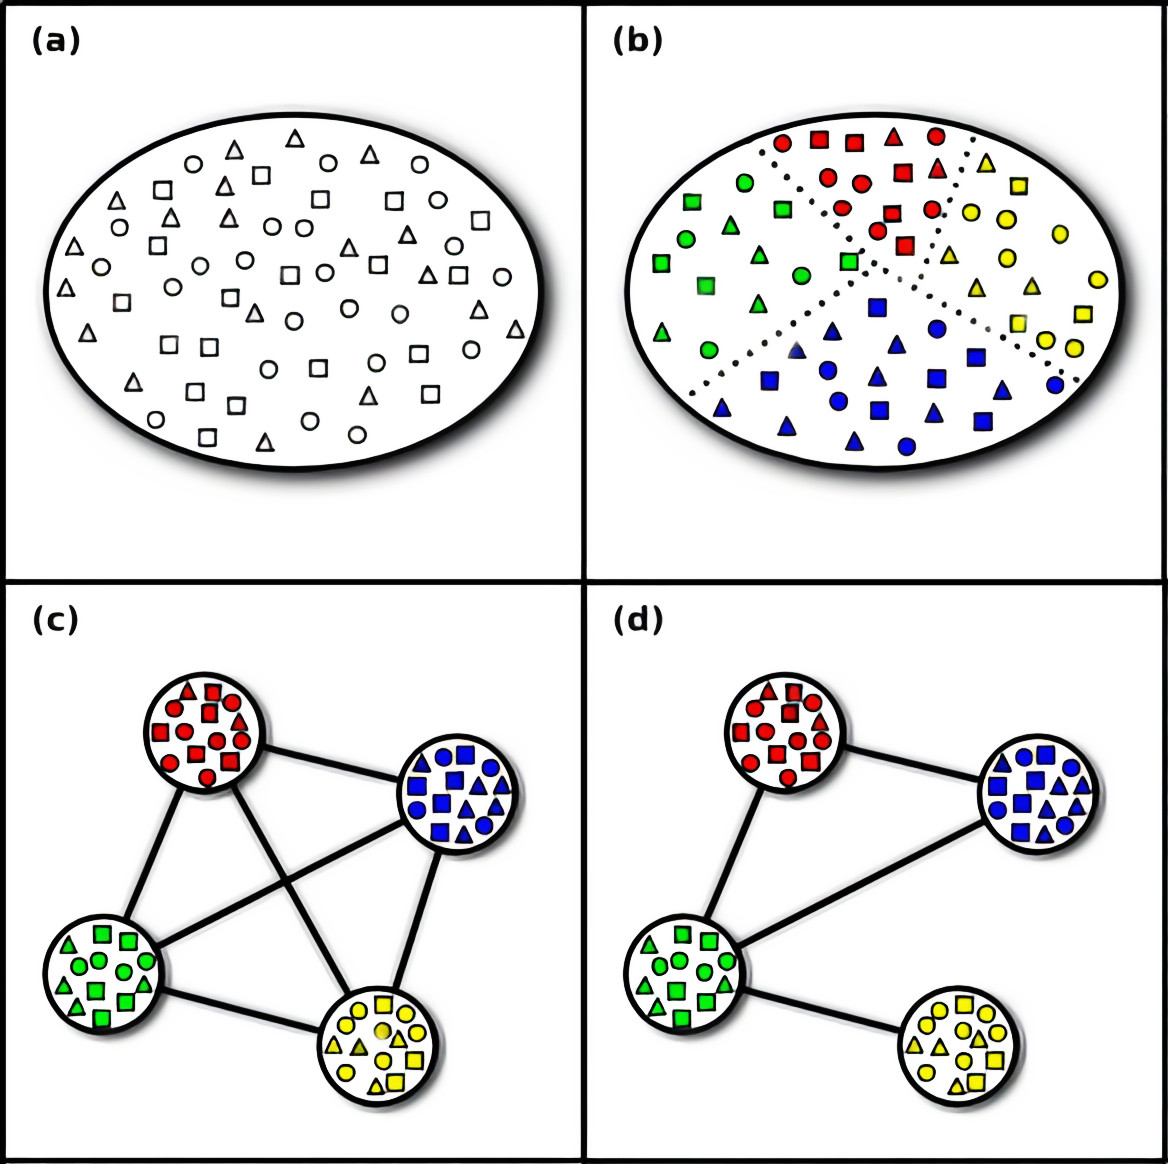
\includegraphics[scale=0.22]{./img/dif_populacao.jpg}}
    \label{fig:dif_populacao}
\end{figure}

Em situações reais, interações entre um número finito de indivíduos podem estar sujeitas a restrições topológicas, nas quais jogadores irão interagir somente com um número reduzido de indivíduos próximos de acordo com essa topologia. Nesse contexto, Madeo e Mocenni \cite{madeo2015} introduziram um modelo que estende a teoria dos jogos evolucionários para redes finitas, representadas por grafos que descrevem as conexões entre os jogadores. Grafos são estruturas formadas por vértices e arestas, que são pares de vértices, e são usados para descrever os mais variados tipos de redes. Iremos considerar cada subpopulação como um jogador vértice, que usa a estratégia mista corresponde à distribuição de estratégias puras da subpopulação. Podemos ver abaixo na figura \ref{fig:dif_populacao}(c) um jogo em rede equivalente ao jogo multipopulação em \ref{fig:dif_populacao}(b), descrito através de um grafo completo, onde todos vértices estão conectados entre si.

Na figura \ref{fig:dif_populacao}(d) temos um jogo em redes finitas, onde nem todos jogadores vértices estão conectados devido às restrições topológicas. Uma aresta entre dois jogadores indica que eles interagem, porém um jogador pode considerar alguma interação como mais importante que as outras e dois jogadores podem ter percepções diferentes sobre a importância daquela interação e, até mesmo, a interação ser unilateral. Portanto, os grafos serão, em geral, direcionados e ponderados, onde um peso positivo na aresta indica a importância dada pelo jogador de origem para aquela interação.

Formalmente, seja $\G$ um grafo direcionado e ponderado com $N<\infty$ vértices (de ordem $N$) e $\V=\{1,2,\dots,N\}$ o seu conjunto de vértices. O grafo $\G$ é completamente descrito por sua matriz de adjacências $A\in\R^{N\times N}_{\geq0}$. Mais precisamente, sempre que há uma aresta que sai do jogador $v$ e termina no jogador $u$ a entrada $a_{v,u}$ da matriz será o peso que $v$ dá para a interação com $u$. Quando $a_{v,u}>0$ e $a_{u,v}=0$, somente $v$ receberá um pagamento na interação com $u$. Por fim, se $a_{v,u}=a_{u,v}=0$ quer dizer que $v$ e $u$ não interagem entre si. Além disso, nesse modelo assumimos que não existem loops, ou seja, arestas que saem de $v$ e terminam em $v$. Em outras palavras, temos $a_{v,v}=0, \forall v\in\V$.

A seguir iremos definir o pagamento e a equação de replicação para jogos evolucionários em redes finitas e listar algumas propriedades e definições importantes para o trabalho.

% -- % -- % -- %

\section{Pagamento e Equilíbrio de Nash em Redes Finitas}

A cada instante dois jogadores vértices que estão conectados são selecionados para jogar entre si. Um replicador de cada vértice é escolhido aleatoriamente para o jogo e o pagamento é o sucesso reprodutivo, de maneira análoga aos jogos multipopulação que vimos até o momento. Assim, o pagamento esperado de um jogador vértice depende das interações com todos os jogadores com os quais ele está conectado, a sua vizinhança. Dado um perfil de estratégias $\BS{X}\in\Delta$, podemos definir o pagamento esperado de $v\in\V$ como
\begin{equation}
    \label{pagtoWS}
    \pi^\G_v(\BS{X})= \BS{x_v} B_v \BS{k_v}(\BS{X})
\end{equation}
onde $B_v$ é a matriz de pagamentos de $v$ para o jogo e $\BS{k_v}(\BS{X})=\frac{1}{d_v}\sum^N_{u=1} a_{v,u} \BS{x_u}$, com $d_v=\sum^N_{u=1} a_{v,u}$, o grau do vértice $v$. Note que o pagamento esperado nada mais é que a soma do pagamento de todas interações dois à dois ponderada pelo peso das arestas do grafo. Para simplificar a notação, defina o pagamento esperado de $v$ ao usar a estratégia pura $s\in S$ por $p^\G_{v,s}=\pi^\G_v(\BS{e_s},\BS{X_{-v}})$ e o pagamento esperado de $v$ ao usar a estratégia mista $\BS{x_v}\in\Delta_M$ por $\phi^\G_v=\pi^\G_v(\BS{x_v},\BS{X_{-v}})$. 

Perceba que a estrutura do grafo está embutida na função de pagamentos e, portanto, a definição de equilíbrio de Nash é equivalente à definição \ref{DefEqNashClassico}, porém também pode ser definido em função do pagamento esperado para estratégias puras da seguinte maneira.

\begin{definition}
    \label{defEqNashEstPura}
    O conjunto de equilíbrio de Nash é definido como sendo
    \begin{equation*}
        \Theta^{NE}=\{\BS{X}\in\Delta\;\mid\;  \forall v,\forall x_{v,s}>0, p^\G_{v,s}=p^\G_{v,s'}, \forall x_{v,s'}>0 \;\;\text{e}\;\; p^\G_{v,s}\geq p^\G_{v,s'}, \forall x_{v,s'}=0\}
    \end{equation*}
    E o conjunto de equilíbrio de Nash estrito é dado por
    \begin{equation*}
        \Theta^{NES}=\{\BS{X}\in\Delta\;\mid\;  \forall v,\forall x_{v,s}>0, p^\G_{v,s}>p^\G_{v,s'}, \forall x_{v,s'}=0\}.
    \end{equation*}
\end{definition}

Em outras palavras, um perfil de estratégias é um equilíbrio de Nash se, para todo jogador, nenhuma das estratégias presentes no perfil possui vantagem sobre as demais e a aptidão das estratégias que não estão presentes no perfil é menor ou igual que a aptidão das demais. Novamente, equilíbrio é estrito se a desigualdade for estrita.

% -- % -- % -- %

\section{Equação de Replicação}

Usando a função de pagamento definida em $\eqref{pagtoWS}$ a equação de replicação multipopulação pode ser estendida para jogos em grafos \cite{madeo2015}, resultando no seguinte problema de Cauchy.

\begin{equation}
    \label{EqRepEGN}
    \left\{\begin{matrix*}[l]
        \dot{x}_{v,s}(t)=x_{v,s}(t)\left(\rho^\G_{v,s}(t)-\phi^\G_v(t)\right)\\
        x_{v,s}(0)=c_{v,s}
    \end{matrix*}\right.
    \;\;\forall v\in\V,s\in S
\end{equation}
onde $\BS{x_v}(0)=[c_{v,1}\dots c_{v,M}]\in\Delta_M$ é a condição inicial do jogador $v$.

A equação de replicação para jogos em grafos também é invariante em $\Delta$. Além disso, estratégias puras e equilíbrios de Nash são estados estacionários de $\eqref{EqRepEGN}$ e um perfil de estratégias $\BS{X^*}\in\text{int}(\Delta)$ é um estado estacionário se, e somente se, $\BS{X^*}\in\Theta^{NE}$.

O teorema a seguir mostra que a equação de replicação clássica pode ser obtida como um caso especial da equação de replicação em grafos. Para isso, mostraremos que as soluções da equação em grafos $\eqref{EqRepEGN}$ e da equação clássica $\eqref{eqRep}$ são equivalentes sob algumas hipóteses.

\begin{theorem}[Madeo e Mocenni \cite{madeo2015}]
    \label{TeoEquivalenciaEGN}
    Seja $\BS{X}(t)=\{\BS{x}_1(t)\dots\BS{x}_N(t)\}$ a única solução do problema de Cauchy $\eqref{EqRepEGN}$, onde $x_{v,s}(0)=c_s, \forall v$. Assuma também que $B_v=B, \forall v$. Seja $\BS{y}(t)$ a única solução do problema de Cauchy $\eqref{eqRep}$, com $y_s(0) = c_s$. Então, $\BS{x_v}(t)=\BS{y}(t), \forall v, \forall t\geq 0$.
\end{theorem}
\begin{proof}[Dem.:]
    Seja $\BS{X}(t)$ e $\BS{y}(t)$ como definido nas hipóteses. Tome um perfil de estratégias $\BS{Y}$ no qual a distribuição de estratégias de todos os $N$ jogadores é dada por $\BS{y}(t)$, a solução do problema $\eqref{eqRep}$. Com isso, temos
    \begin{equation*}
        \BS{k_v}(\BS{Y})=\frac{1}{d_v}\sum^N_{u=1}a_{v,u}\BS{y}(t)=\BS{y}(t)
    \end{equation*}
    ou seja, como todos usam a mesma estratégia $\BS{y}(t)$, a média ponderada de todas interações é, também, $\BS{y}(t)$. Assim, os pagamentos de todos jogadores serão dados por
    \begin{equation*}
    \begin{split}
        p^\G_{v,s}&=\BS{e_s}B\BS{k}_v(\BS{Y})=\BS{e_s}B\BS{y}=\pi_s\\
        \phi^\G_{v}&=\BS{x_v}B\BS{k}_v(\BS{Y})=\BS{y}B\BS{y}=\phi
    \end{split}
    \end{equation*}
    Logo, a equação de replicação em grafos aplicada ao perfil de estratégias $\BS{Y}$ é dada por
    \begin{equation*}
        \dot{y}_{v,s}=y_{v,s}(p^\G_{v,s}-\phi^\G_v)=y_s(\pi_s-\phi)=\dot{y}_s
    \end{equation*}
    Então, $\BS{Y}(t)$ é uma solução da equação $\eqref{EqRepEGN}$ e, pela unicidade da solução do problema de Cauchy $\eqref{EqRepEGN}$, temos que $\BS{x_v}(t)=\BS{y}(t),\forall v,\forall t\geq 0$. Em outras palavras, dados $\BS{X}(t)$ e $\BS{y}(t)$ como definido nas hipóteses, a equação de replicação em grafos é equivalente a equação de replicação clássica.
\end{proof}


% Hiper-racionalidade
\chapter{Hiper-racionalidade} \label{chap:hiperRacionalidade}

Um ponto central da teoria dos jogos clássica é a hipótese de racionalidade. É através dela que os indivíduos são capazes de escolher a estratégia que mais lhe beneficiam e que dilemas interessantes, como o dilema do prisioneiro, surgem. Nos jogos evolucionários nós assumimos que cada indivíduo carrega um fenótipo que é transmitido aos seus descendentes, não havendo a hipótese de racionalidade. Já nos jogos multipopulação, ou em grafos, temos um comportamento análogo aos jogos com $N$ jogadores da teoria clássica, onde uma população, ou jogador vértice, maximiza sua utilidade através do processo evolutivo, imitando a racionalidade.

\begin{definition}
    \label{defRacionalidade}
    Um indivíduo é dito racional se, dado um conjunto de possíveis resultados $\Omega=\{\omega_1,\omega_2,\omega_3,\dots\}$, ele possui preferências que satisfazem as seguintes condições:
    \begin{itemize}
        \item[1)] (Completude) Temos $\omega_1\preceq\omega_2$ ou $\omega_2\preceq\omega_1$;
        \item[2)] (Transitividade) Se $\omega_1\preceq\omega_2$ e $\omega_2\preceq\omega_3$, então $\omega_1\preceq\omega_3$.
    \end{itemize}
\end{definition}

Diversos resultados de economia experimental mostraram que a hipótese de racionalidade não descreve bem o comportamento humano. Por exemplo, muitas vezes um indivíduo irá preferir $A$ ao invés de $B$, $B$ ao invés de $C$ e $C$ ao invés de $A$ \cite{sep-game-evolutionary}. Essa falha na transitividade não ocorreria se o indivíduo possuísse um conjunto de preferências bem definido e consistente. Para descrever melhor comportamentos humanos como altruísmo, devoção, desconfiança e ciúmes, podemos considerar duas classes de preferências: pessoal e social. A preferência pessoal busca lucro ou prejuízo para si mesmo, enquanto a preferência social trata do lucro ou prejuízo para pelo menos um dos demais indivíduos, assim um indivíduo poderá escolher entre sua preferência pessoal, social ou ambas. Com isso, um jogador terá um novo ranqueamento de preferências, chamado de hiperpreferências \cite{askari2019behavioral}. Formalmente, definimos $\Omega_v=\{\omega_1,\omega_2,\dots,\omega_v,\dots,\omega_N\}$ como um conjunto de escolhas do indivíduo $v$ para a interação com cada indivíduo $i\in\{1,2,\dots,N\}$, tomando dois conjuntos de escolhas $\Omega$ e $\Omega'$, podemos definir as hiperpreferências do indivíduo como segue.

\begin{definition}[Askari, Gordji e Park \cite{askari2019behavioral}]
    \label{defHiperPreferencias}
    As hiperpreferências do jogador $v$ são uma relação sobre o conjunto de todas as escolhas do indivíduo na qual, dados $\Omega_v$ e $\Omega_v'$, temos $\Omega_v\preceq\Omega_v'$ se, para todo $u\in\{1,2,\dots,N\}$, $\omega_u\preceq\omega_u'$ ou $\omega_u'\preceq\omega_u$ baseado na preferência pessoal, social ou ambas de $v$.
\end{definition}

Note que essa relação não é necessariamente completa nem transitiva, porém um indivíduo, quando forçado a escolher entre dois conjuntos de escolhas, sempre terá predileção por um. Essa predileção depende nas condições da interação, comportamento, crenças e quaisquer outros valores que o indivíduo venha a ter. Por conta disso, as hiperpreferências nos ajudam a obter condições mais realistas para a tomada de decisão do indivíduo \cite{askari2019behavioral}.

\begin{definition}[Askari, Gordji e Park \cite{askari2019behavioral}]
    Um indivíduo é dito hiper-racional se ele é racional (\ref{defRacionalidade}) e suas hiperpreferências satisfazem ao menos uma das seguintes condições:
    \begin{itemize}
        \item [1)] O indivíduo faz sua escolha baseado em sua preferência pessoal;
        \item [2)] O indivíduo faz sua escolha baseado em sua preferência social.
    \end{itemize}
\end{definition}

Perceba que todo indivíduo hiper-racional é racional, mas nem todo indivíduo racional é hiper-racional. Podemos concluir que um indivíduo é hiper-racional se ele considera o pagamento dos demais envolvidos em suas interações, portanto ele nem sempre é capaz de identificar qual ação irá maximizar seu benefício, mas pode fazer uma escolha que maximiza o benefício dos demais agentes envolvidos. Um agente hiper-racional escolhe sua ação baseado em suas hiperpreferências, apesar de não ter conhecimento das hiperpreferências dos demais, ou seja, agentes hiper-racionais não possuem informação completa. Essa característica é muito importante para a dinâmica entre jogadores hiper-racionais e será mais explorada nas próximas seções.

Como dito anteriormente, a hiper-racionalidade permite que alguns comportamentos humanos possam ser expressados por agentes hiper-racionais. Um agente altruísta busca maximizar o benefício de vários dos agentes envolvidos, enquanto um agente devoto a um outro indivíduo busca maximizar o benefício deste indivíduo, mesmo que isso diminua o seu benefício pessoal, e um agente ciumento, ou invejoso, busca diminuir o benefício de agentes bem sucedidos quando ele não consegue aumentar o seu próprio.

Agora que temos o conceito de escolha hiper-racional definido nosso objetivo é aplicá-lo como base da teoria de jogos e adaptar a equação de replicação para agentes hiper-racionais. Essa construção e suas consequências serão apresentadas nos próximos capítulos.


% Jogos com Jogadores Hiper-racionais
\chapter{Jogos com agentes hiper-racionais}

Sabemos que agentes hiper-racionais podem ter como objetivo o lucro ou prejuízo para si ou qualquer outro jogador envolvido. Para quantificar essas hiperpreferências e aplicá-las no pagamento do jogador nós iremos definir a matriz de preferências $\Rc$, onde a entrada $r_{v,u}\in[-1,1]$ denota a preferência do jogador $v$ pelo jogador $u$ e $r_{v,v}\in[-1,1]$ é preferência de $v$ por si mesmo. Quando $r_{v,u}$ é positivo, o jogador $v$ busca aumentar o lucro do jogador $u$. Quando $r_{v,u}$ é negativo, o jogador $v$ busca diminuir o lucro do jogador $u$. Se $r_{v,u}$ é zero, o jogador $v$ é indiferente quanto ao lucro ou prejuízo de $u$. Além disso, vamos definir que $\Rc$ é linha estocástica em módulo, ou seja, temos que
\begin{equation}
    \sum_{u=1}^N |r_{v,u}| = 1
\end{equation}

Essa hipótese não implica em perda de generalidade, pois, se não fosse, bastaria dividir as entradas de $\Rc$ por essa soma para tornar $\Rc$ linha estocástica em módulo.

Em outras palavras, o pagamento de um jogador hiper-racional é uma média ponderada entre o seu pagamento efetivo e um pagamento virtual proveniente de suas preferências, onde os pesos são as entradas da linha correspondente ao jogador na matriz $\Rc$. Com isso, dado um perfil de estratégias $\BS{X}=\{\BS{x_1},\BS{x_2},\dots,\BS{x_N}\}\in\Delta$ e as matrizes de pagamento $B_v,\forall v\in\V$, podemos definir o pagamento para agentes hiper-racionais como segue.

\begin{equation}
    \label{defPgtoHR}
    \pi^{\mathcal{H}}_v(\BS{X})=r_{v,v}\left[\BS{x_v} B_v \left(\frac{1}{N-1}\sum_{\substack{u=1\\u\neq v}}^N \BS{x_u}\right)\right] + \sum_{\substack{u=1\\u\neq v}}^N r_{v,u} \left(\BS{x_u} B_u \BS{x_v}\right)
\end{equation}

Temos agora um novo termo sendo somado na nossa função de pagamento, é o pagamento de $u$ no jogo clássico entre $u$ e $v$. Dizemos que esse termo é o pagamento de $u$ percebido por $v$ e vamos denotá-lo por

\begin{equation}
    \label{defPgtoPercebido}
    \pi^{\mathcal{H}}_{u,v}(\BS{x_u},\BS{x_v}) = \BS{x_u} B_u \BS{x_v}
\end{equation}

Note que o jogador $v$ não possui informação sobre as preferências de $u$, pois conhece apenas a estratégia mista e a matriz de pagamentos de $u$, além disso, para que $v$ possa estimar o impacto das suas ações no pagamento de $u$, ele assume que $u$ é um jogador racional. Essa assimetria de informação é importante e suas consequências serão discutidas na seção a seguir. 

Definiremos agora o hiperequilíbrio, que usa o pagamento $\eqref{defPgtoHR}$. Esse equilíbrio é análogo ao equilíbrio de Nash, definido em \ref{DefEqNashClassico}, porém usa o pagamento hiper-racional e tem as hiperpreferências do jogador imbuída na sua formulação. Essa distinção permite analisar separadamente os novos equilíbrios introduzidos pelas hiperpreferências dos jogadores \cite{askari2019behavioral}.

\begin{definition}
    \label{defHiperEq}
    Dado um perfil de estratégias $\BS{X^*}=(\BS{x}^*_{1},\BS{x}^*_{2},\dots,\BS{x}^*_{N})\in\Delta$ e uma matriz de preferências $\Rc$, dizemos que $\BS{X^*}$ é um hiperequilíbrio se
    \begin{equation*}
        \pi^{\mathcal{H}}_v(\BS{x}^*_v,\BS{X}^*_{-i})\geq \pi^{\mathcal{H}}_v(\BS{x}_v,\BS{X}^*_{-i})
    \end{equation*}
    para todo $\BS{x}_v\in\Delta_{M_i}$. Se a desigualdade for estrita, dizemos que $\boldsymbol{X^*}$ é um hiperequilíbrio estrito.
\end{definition}

%\begin{definition}[\citeauthor{askari2019behavioral}, 2019]
%    Um perfil de estratégias $\BS{X^*}$ é um hiper equilíbrio se, para todo jogador $v\in\V$ e todo $x_v\in\Delta_M$, temos
%    \begin{equation}
%        \pi^{\mathcal{H}}_{u,v}(\BS{x^*_u},\BS{x^*_v}) \geq \pi^{\mathcal{H}}_{u,v}(\BS{x^*_u},\BS{x_v})
%    \end{equation}
%    para todo jogador $u\in\V,u\neq v$ tal que $r_{v,u}>0$ e
%    \begin{equation}
%        \pi^{\mathcal{H}}_{u,v}(\BS{x^*_u},\BS{x^*_v}) \leq \pi^{\mathcal{H}}_{u,v}(\BS{x^*_u},\BS{x_v})
%    \end{equation}
%    para todo jogador $u\in\V,u\neq v$ tal que $r_{v,u}<0$.
%\end{definition}
%Em outras palavras, um hiper equilíbrio é um estado no qual o jogador não consegue alterar unilateralmente sua estratégia para aumentar ou diminuir o pagamento dos jogadores presentes em suas preferências. Nem todo jogo hiper-racional possui um hiper equilíbrio e nem todo hiper equilíbrio é também um equilíbrio de Nash. Veremos mais sobre isso com exemplos nos próximos capítulos.

Na próxima seção iremos analisar um jogo que possui um hiper equilíbrio diferente do equilíbrio de Nash esperado por um jogador racional, mostrando na prática o motivo de haver essa separação nas definições.

% -- % -- % -- %

\section{Assimetria de informação no jogo hiper-racional}

Num primeiro momento, pode-se pensar que as preferências sociais podem ser descritas através de mudanças na matriz de pagamentos do jogador, porém o exemplo a seguir mostra que isso não é possível, pois um jogador não possui informação sobre as preferências dos demais. Considere um jogo com dois jogadores hiper-racionais, $v_1$ e $v_2$, com a matriz de pagamentos abaixo.
\begin{table}[h]
\begin{center}
    \begin{tabular}{ccccc}
        & & \multicolumn{3}{c}{$v_2$} \\
        & & $X$ & $Y$ & $Z$ \\ \cline{3-5} 
        \multirow{3}{*}{$v_1$} & \multicolumn{1}{c|}{$A$} & \multicolumn{1}{l|}{$(1,3)$} & \multicolumn{1}{l|}{$(2,4)$} & \multicolumn{1}{l|}{$(0,6)$} \\ \cline{3-5} 
        & \multicolumn{1}{c|}{$B$} & \multicolumn{1}{l|}{$(2,2)$}  & \multicolumn{1}{l|}{$(2,2)$} & \multicolumn{1}{l|}{$(1,1)$}  \\ \cline{3-5} 
        & \multicolumn{1}{l|}{$C$} & \multicolumn{1}{l|}{$(1,1)$}  & \multicolumn{1}{l|}{$(1,1)$} & \multicolumn{1}{l|}{$(0,2)$} \\ \cline{3-5} 
    \end{tabular}
    \caption{Matriz de pagamentos do jogo exemplo.}
    \label{JogoHRassimetrico}
\end{center}
\end{table}

O jogador $v_1$ é altruísta, ou seja, ele se importa com o pagamento do seu adversário, mesmo que resulte em um pagamento efetivo menor para si próprio, porém $v_2$ age como um jogador racional clássico, se importando apenas com seu pagamento. A matriz de preferências é como segue.
\begin{equation}
    \label{matrizPrefAssimetrico}
    \mathcal{R}=
    \begin{bmatrix}
        \frac{1}{2} & \frac{1}{2}\\ 
        0 & 1 
    \end{bmatrix}
\end{equation}

Assim, enquanto $v_2$ joga usando a matriz \eqref{JogoHRassimetrico}, $v_1$ joga usando uma matriz de pagamentos virtual que leva em consideração suas preferências. O pagamento virtual de $v_1$ é dado pela matriz abaixo, onde seu pagamento foi calculado de acordo com a equação \eqref{defPgtoHR}.

\begin{table}[h]
\begin{center}
    \begin{tabular}{ccccc}
        & & \multicolumn{3}{c}{$v_2$} \\
        & & $X$ & $Y$ & $Z$ \\ \cline{3-5} 
        \multirow{3}{*}{$v_1$} & \multicolumn{1}{c|}{$A$} & \multicolumn{1}{l|}{$(2,3)$} & \multicolumn{1}{l|}{$(3,4)$} & \multicolumn{1}{l|}{$(3,6)$} \\ \cline{3-5} 
        & \multicolumn{1}{c|}{$B$} & \multicolumn{1}{l|}{$(2,2)$}  & \multicolumn{1}{l|}{$(2,2)$} & \multicolumn{1}{l|}{$(1,1)$}  \\ \cline{3-5} 
        & \multicolumn{1}{l|}{$C$} & \multicolumn{1}{l|}{$(1,1)$}  & \multicolumn{1}{l|}{$(1,1)$} & \multicolumn{1}{l|}{$(1,2)$} \\ \cline{3-5} 
    \end{tabular}
    \caption{Matriz de pagamentos virtual de $v_1$.}
    \label{PagVirtualV1}
\end{center}
\end{table}

Do ponto de vista de $v_2$, podemos ver que a estratégia $B$, de $v_1$, domina fracamente todas as demais estratégias e, portanto, $v_2$ terá de decidir entre as estratégias $X$ e $Y$, pois são as que lhe dão o maior retorno contra $B$.

\begin{table}[h]
\begin{center}
    \begin{tabular}{cccc}
        & & \multicolumn{2}{c}{$v_2$} \\
        & & $X$ & $Y$ \\ \cline{3-4} 
        $v_1$ & \multicolumn{1}{c|}{$B$} & \multicolumn{1}{l|}{$(2,2)$}  & \multicolumn{1}{l|}{$(2,2)$}  \\ \cline{3-4} 
    \end{tabular}
    \caption{Matriz após a remoção das estratégias dominadas.}
\end{center}
\end{table}

Finalmente, apesar de ambas opções resultarem no mesmo pagamento, $v_2$ irá jogar $Y$, pois possui um melhor pagamento esperado contra $A$ ou $C$. Do ponto de vista de $v_1$, a estratégia $A$ domina fracamente todas as demais e, portanto, será a sua escolha. Assim, o hiperequilíbrio desse jogo é dado pelo perfil $(A,Y)$, com pagamento efetivo $(2,4)$, enquanto os equilíbrios de Nash, esperados por $v_2$, são dados por $(B,Y)$ e $(B,X)$, com pagamento efetivo $(2,2)$.

Além disso, se as preferências pudessem ser simplesmente traduzidas na matriz de pagamento o equilíbrio seria dado pelo perfil $(A,Z)$, pois $v_2$ iria explorar o altruísmo de $v_1$ para obter um pagamento maior para si mesmo. Esse comportamento só acontece por conta da assimetria de informação entre os jogadores. Cada jogador possui um pagamento virtual próprio que influencia suas decisões e, como vimos no exemplo acima, muda o resultado do jogo. Porém, em um jogo iterado, $v_2$ seria capaz de, eventualmente, descobrir e explorar o altruísmo de $v_1$. Esse comportamento é esperado de um jogador racional, que busca o melhor pagamento para si, mas ainda assim o resultado seria diferente dos equilíbrios de Nash do jogo.


% Equação de replicação Hiper-racional em redes finitas
\chapter{Equação de replicação Hiper-racional em redes finitas}

Nos capítulos anteriores nós introduzimos um modelo para jogos evolucionários em redes finitas \cite{madeo2015}, agora iremos modificar a função de pagamento \eqref{defPgtoHR} para que ela comporte jogos em redes finitas e, em sequência, iremos utilizar esse pagamento como base da equação de replicação \eqref{EqRepEGN}.

Primeiramente, dado um perfil de estratégias $\BS{X}\in\Delta$ e um grafo $\G$ descrito por sua matriz de adjacências $A$, vamos relembrar a definição de $\BS{k_v}(\BS{X})$, o jogador virtual da vizinhança de $\BS{X}$.

\begin{equation}
    \BS{k_v}(\BS{X})=\frac{1}{d_v}\sum^N_{u=1} a_{v,u} \BS{x_u}
\end{equation}

Note que estamos usando a vizinhança ponderada por $d_v$, o grau do vértice $v$. Para completar, dadas as matrizes de pagamento $B_v,\forall v\in\V$, e a matriz de preferências $\Rc$, definimos o pagamento esperado de $v$ ao usar a estratégia $\BS{x_v}$ como

\begin{equation}
\begin{split}
    \label{defPgtoEGNHR}
    \pi_v(\BS{x_v},\BS{X_{-v}}) &= r_{v,v}\BS{x_v} B_v \left(\frac{1}{d_v}\sum_{u=1}^N a_{v,u}\BS{x_u}\right)+ \left(\frac{1}{d_{v,r}}\sum_{u=1}^N r_{v,u} a_{v,u} \BS{x_u}B_u\right) \BS{x_v} \\
    &= r_{v,v}\BS{x_v} B_v \BS{k_v}+ \left(\frac{1}{d_{v,r}}\sum_{u=1}^N r_{v,u}a_{v,u}\BS{x_u}B_u\right) \BS{x_v}
\end{split}
\end{equation}
onde $d_{v,r}$ é o grau de preferências do vértice $v$, a soma dos pesos das arestas para os vértices que $v$ possui preferência. Por conveniência usaremos somente $\pi_v$ para denotar esse pagamento, pois a partir de agora esse será o pagamento utilizado em todos nossos cálculos, exceto quando explicitamente dito o contrário. Da mesma forma, iremos reutilizar a notação de $\rho_{v,s}=\pi_v(\BS{e_s},\BS{X_{-v}})$ e $\phi_v=\pi_v(\BS{x_v},\BS{X_v})$, o pagamento de $v$ ao usar a estratégia pura e $s$ e o pagamento esperado de $v$ ao usar $\BS{x_v}$, respectivamente.

Finalmente, a equação de replicação hiper-racional para jogos em redes finitas é dada, em sua forma extensa, por
\begin{equation}
    \label{defEqRepHR}
    \Dot{x}_{v,s}(t)= \!\begin{multlined}[t]
        x_{v,s}(t)\left[r_{v,v}\BS{e_s} B_v \BS{k_v}(t)+ \left(\frac{1}{d_{v,r}}\sum_{u=1}^Nr_{v,u}a_{v,u} \BS{x_u}(t)B_u\right)\BS{e_s} \right. \\
        \left. -r_{v,v}\BS{x_v}(t) B_v \BS{k_v}(t) -\left(\frac{1}{d_{v,r}}\sum_{u=1}^N r_{v,u}a_{v,u}\BS{x_u}(t)B_u\right) \BS{x_v}(t)\right]
    \end{multlined}
\end{equation}

Para facilitar a leitura, podemos reorganizá-la da seguinte forma
\begin{equation}
    \Dot{x}_{v,s}(t)= \!\begin{multlined}[t]
        x_{v,s}(t)\Biggl[ r_{v,v}\left(\BS{e_s} B_v \BS{k_v}(t)-\BS{x_v}(t) B_v \BS{k_v}(t)\right) \\
        +\frac{1}{d_{v,r}}\sum_{u=1}^N r_{v,u}a_{v,u}
        \left(\BS{x_u}(t) B_u \BS{e_s}-\BS{x_u}(t) B_u \BS{x_v}(t)\right)\Biggr]
    \end{multlined}
\end{equation}

A primeira parte da equação é a mesma equação de replicação definida em $\eqref{EqRepEGN}$, enquanto a segunda parte é a diferença entre o pagamento percebido de $u$ por $v$ ao usar a estratégia $s$ e ao usar a estratégia $x_v$. Diremos que essas são, respectivamente, a parte pessoal e parte social da equação de replicação hiper-racional e denotamos
\begin{equation}
    \psi_{v,s}(t)=r_{v,v}\left(\BS{e_s} B_v \BS{k_v}(t)-\BS{x_v}(t) B_v \BS{k_v}(t)\right)
\end{equation}
como a parte pessoal da equação, e
\begin{equation}
    \gamma_{v,s}(t)=\frac{1}{d_{v,r}}\sum_{u=1}^N r_{v,u}a_{v,u}
                    \left(\BS{x_u}(t) B_u \BS{e_s}-\BS{x_u}(t) B_u \BS{x_v}(t)\right)
\end{equation}
como a parte social da equação. Assim, a nossa equação de replicação pode ser apresentada na sua forma reduzida como
\begin{equation}
    \label{EqReduzida}
    \Dot{x}_{v,s}(t)=x_{v,s}(t)\left(\psi_{v,s}(t)+\gamma_{v,s}(t)\right)
\end{equation}

A seguir, iremos demonstrar algumas importantes propriedades da equação $\eqref{defEqRepHR}$ e as hipóteses necessárias para que ela seja equivalente às demais equações de replicação apresentadas neste trabalho.

% -- % -- % -- %

\section{Existência e unicidade da solução}

Nosso objetivo é provar que a equação $\eqref{defEqRepHR}$ satisfaz as hipóteses do teorema \ref{teoExistUnic} e, portanto, possui uma única solução para cada condição inicial dada. Precisamos apenas mostrar que $\eqref{defEqRepHR}$ é Lipschitz, pois pela compacidade de $\Delta_M$ teremos que $\eqref{defEqRepHR}$ também é contínua e limitada em $\Delta_M$. Para isso, dados $\BS{x},\BS{y}\in\Delta$, defina $F_v(\BS{x})=\left[ \dot{\BS{x}}_{v,1} \dots \dot{\BS{x}}_{v,s} \dots \dot{\BS{x}}_{v,M}\right]^T$, para todo $v\in\V$ e $s\in S$, e a função $c(t)=\BS{y}+t(\BS{x}-\BS{y})$ de forma que, usando o teorema fundamental das integrais de linha \ref{teoGradiente}, obtemos
\begin{equation}
    F_v(\BS{x})-F_v(\BS{y})=F_v(c(1))-F_v(c(0))=\int_0^1 \nabla F_v(c(t)) \; (\BS{x}-\BS{y}) \; dt , \forall v\in\V
\end{equation}
Assim, temos
\begin{equation}
    \label{ineqLipschitz}
    |F_v(\BS{x})-F_v(\BS{y})|\leq\int_0^1 \|\nabla F_v(c(t))\| \; \|\BS{x}-\BS{y}\| \; dt, \forall v\in\V
\end{equation}
onde
\begin{equation}
    \nabla F_v(\BS{x})=\left[ \pdv{F_v}{x_{v,1}} \dots \pdv{F_v}{x_{v,s}} \dots \pdv{F_v}{x_{v,M}} \right]^T
\end{equation}

Agora vamos analisar as entradas de $\nabla F_v(\BS{x})$ para tentar limitar o valor de seu módulo e encontrar a constante de Lipschitz $L$ para a equação de replicação hiper-racional. Assim, para todo $s\in S$ e $v\in\V$, onde $b_{v,s,t}$ é a entrada $(i,j)$ da matriz de pagamentos $B_v$, temos
\begin{equation}
    \left\|\pdv{F_v}{x_{v,s}}\right\| = \!\begin{multlined}[t]
        \Biggl| \frac{r_{v,v}}{d_v} \left( 
        \sum^M_{l=1}\sum^N_{u=1} a_{v,u}b_{v,s,l}x_{u,l} - \sum^M_{l=1}\sum^M_{k=1}\sum^N_{u=1} a_{v,u}x_{v,k}b_{v,k,l}x_{u,l} \right) \\
        + \frac{1}{d_{v,r}}\sum^N_{u=1}r_{v,u}a_{v,u}\left( \sum^M_{k=1}x_{u,k}b_{u,k,s} - \sum^M_{l=1}\sum^M_{k=1}x_{u,k}b_{u,k,l}x_{v,l}\right) \\
        - \frac{r_{v,v}}{d_v}\left( \sum^M_{l=1}\sum^N_{u=1} a_{v,u}x_{v,s}^2b_{v,s,l}x_{u,l} \right)  \\
        - \frac{1}{d_{v,r}}\sum^N_{u=1}r_{v,u}a_{v,u}
        \left( \sum^M_{k=1}x_{u,k}b_{u,k,s}x_{v,s}^2\right) \Biggr|
    \end{multlined}
\end{equation}
Pela desigualdade triangular, temos
\begin{equation}
\begin{split}
    \left\|\pdv{F_v}{x_{v,s}}\right\| \leq &
    \left| \frac{r_{v,v}}{d_v}\sum^M_{l=1}\sum^N_{u=1} a_{v,u}b_{v,s,l}x_{u,l} \right| + \left| \frac{r_{v,v}}{d_v}\sum^M_{l=1}\sum^M_{k=1}\sum^N_{u=1} a_{v,u}x_{v,k}b_{v,k,l}x_{u,l} \right| \\
    &+ \left|\frac{1}{d_{v,r}}\sum^N_{u=1} \sum^M_{k=1} r_{v,u}a_{v,u} x_{u,k}b_{u,k,s} \right| \\&+ 
    \left|\frac{1}{d_{v,r}}\sum^N_{u=1}\sum^M_{l=1}\sum^M_{k=1} r_{v,u}a_{v,u}x_{u,k}b_{u,k,l}x_{v,l}\right| \\&+
    \left|\frac{r_{v,v}}{d_v} \sum^M_{l=1}\sum^N_{u=1} a_{v,u}x_{v,s}^2b_{v,s,l}x_{u,l} \right| \\
    &+ \left| \frac{1}{d_{v,r}}\sum^N_{u=1}\sum^M_{k=1} r_{v,u}a_{v,u}x_{u,k}b_{u,k,s}x_{v,s}^2\right|
\end{split}
\end{equation}
Para simplificar, tome $b=\max\{b_{v,k,l}\},\forall v\in\V$ e $k,l\in S$, e lembre-se que $\BS{x_v}\in\Delta_M$, portanto $\sum_{k=1}^M x_{v,s}=1,\forall v\in\V$. Além disso, assumimos que $r_{v,u}\in[0,1]$ para todo $v,u\in\V$, porém o resultado ainda vale para valores em $[-1,1]$, basta tomar o módulo de cada $r_{v,u}$. Então podemos reescrever a equação acima da seguinte maneira,
\begin{equation}
    \left\|\pdv{F_v}{x_{v,s}}\right\| \leq \!\begin{multlined}[t]
        \left| r_{v,v} N b \right| +
        \left|r_{v,v} N b \right| +
        \left|1-r_{v,v}\right| \left| N b \right| \\ + 
        \left|1-r_{v,v}\right| \left| N b \right| +
        \left|r_{v,v} N b x_{v,s}^2 \right|
        +  \left|1-r_{v,v}\right| \left| N b x_{v,s}^2\right|
    \end{multlined}
\end{equation}
Por fim, utilizando o fato de que $x_{v,s}^2\leq 1$, concluímos que
\begin{equation}
\begin{split}
    \left\|\pdv{F_v}{x_{v,s}}\right\| &\leq \!\begin{multlined}[t]
        \left| r_{v,v} N b \right| +
        \left|r_{v,v} N b \right| +
        \left|1-r_{v,v}\right| \left| N b \right| \\+ 
        \left|1-r_{v,v}\right| \left| N b \right| +
        \left|r_{v,v} N b \right| +
        \left|1-r_{v,v}\right| \left| N b\right|
    \end{multlined}\\
    &\leq 3 N b
\end{split}
\end{equation}
Com isso, podemos limitar o módulo de $\nabla F_v(\BS{x})$ da seguinte forma
\begin{equation}
    \left\|\nabla F_v(\BS{x})\right\| \leq \sqrt{9MN^2b^2} = 3 N b \sqrt{M} = L
\end{equation}

Finalmente chegamos no resultado desejado, pois ao substituir o resultado acima na equação $\eqref{ineqLipschitz}$, concluímos
\begin{equation}
    \|F_v(x)-F_v(y)\|\leq L \int_0^1 \|x-y\| \; dt = L\|x-y\|,\forall v\in\V
\end{equation}
Portanto, temos que $F_v$ é de Lipschitz e satisfaz todas as condições do teorema de existência e unicidade da solução \ref{teoExistUnic}.

% -- % -- % -- %

\section{Invariância de $\Delta_M$}

Suponha que $\BS{x_v}(t)\in\Delta_M$ é a única solução do problema $\eqref{EqRepEGN}$ obtida ao tomar $c_v\in\Delta_M$. Suponha também que existe um instante $t_1$ tal que $x_{v,s}(t_1)<0$. Pela continuidade de todas as componentes da solução, temos que existe um $t_2<t_1$ tal que $x_{v,s}(t_2)=0$. Pela equação $\eqref{defEqRepHR}$, temos que $\Dot{x}_{v,s}(t_2)=0$ e, portanto, $x_{v,s}(t_3)=0,\forall t_3>t_2$. Pela unicidade da solução, concluímos que não há $t_1$ tal que $x_{v,s}(t_1)<0$ e, portanto
\begin{equation}
\label{invariancia1}
    \BS{x_v}(0)\in\Delta_M \Rightarrow \BS{x_v}(t)\geq 0,\forall t>0
\end{equation}

Note que a variação total na distribuição de estratégias de um jogador $v\in\V$ é nula, pois $\sum_{s=1}^M x_{v,s}(t)=1$. De fato,
\begin{equation}
    \sum^M_{s=1}\Dot{x}_{v,s}= \!\begin{multlined}[t]
        \sum^M_{s=1}x_{v,s}\Biggl[
        r_{v,v}\BS{e_s} B_v \BS{k_v}+\left(\frac{1}{d_{v,r}}\sum_{u=1}^N 
        r_{v,u}a_{v,u}\BS{x_u} B_u \right) \BS{e_s} \\
        -r_{v,v}\BS{x_v} B_v \BS{k_v}-\left(\frac{1}{d_{v,r}}\sum_{u=1}^N 
        r_{v,u}a_{v,u}\BS{x_u} B_u\right) \BS{x_v}
        \Biggr]
    \end{multlined}
\end{equation}

Que pode ser simplificada da seguinte maneira
\begin{equation}
    \sum^M_{s=1}\Dot{x}_{v,s}= \!\begin{multlined}[t]
        r_{v,v}\left[\sum^M_{s=1}x_{v,s}\BS{e_s} B_v \BS{k_v}-\BS{x_v} B_v \BS{k_v} \sum^M_{s=1}x_{v,s}\right]\\
        +\frac{1}{d_{v,r}}\sum_{u=1}^N r_{v,u}a_{v,u}\left[\BS{x_u} B_u \sum^M_{s=1} x_{v,s} \BS{e_s}
        -x_u^TB_u x_v\sum^M_{s=1}x_{v,s}
        \right]
    \end{multlined}
\end{equation}

Finalmente, temos
\begin{equation}
    \sum^M_{s=1}\Dot{x}_{v,s}= \!\begin{multlined}[t]
        r_{v,v}\left[\BS{x_v} B_v \BS{k_v} - \BS{x_v} B_v \BS{k_v}\right] \\
        +\frac{1}{d_{v,r}}\sum_{u=1}^N r_{v,u}a_{v,u}\left[\BS{x_u} B_u \BS{x_v}
        -\BS{x_u} B_u \BS{x_v}
        \right] = 0
    \end{multlined}
\end{equation}

Isso significa que
\begin{equation}
\label{invariancia2}
    \sum^M_{s=1}x_{v,s}(t)=\sum^M_{s=1}x_{v,s}(0),\forall t>0,\forall v\in\V
\end{equation}

Portanto, tomando $\BS{x}_v(0)\in\Delta_M$ e usando os resultados $\eqref{invariancia1}$ e $\eqref{invariancia2}$, concluímos que
\begin{equation}
    \label{invariancia}
    \forall v\in\V:\BS{x_v}(0)\in\Delta_M\Rightarrow \BS{x_v}(t)\in\Delta_M, \forall t>0
\end{equation}

Em outras palavras, se a condição inicial do problema for uma distribuição de estratégias, então $\BS{x_v}(t)$ será uma distribuição de estratégias $\forall t>0$.

% -- % -- % -- %

\section{Hiperequilíbrios são pontos fixos da equação de replicação hiper-racional em grafos}

Suponha que o perfil de estratégias $\BS{X^*}$ é um hiperequilíbrio, como definido em \ref{defHiperEq}, teremos
\begin{equation}
\begin{split}
    \Dot{x}_{v,s}^*(t)&=x_{v,s}^*(t)\left(\rho_{v,s}^*(t)-\phi_v^*(t)\right)\\
                      &=x_{v,s}^*(t)\left(\pi_v(\BS{e_s},\BS{x^*_{-v}}(t))
                      -\pi_v(\BS{x^*_v}(t),\BS{x^*_{-v}}(t))\right)\\
                      &\leq 0
\end{split}
\end{equation}

Usando o resultado $\eqref{invariancia}$, concluímos que 
\begin{equation}
    \Dot{x}_{v,s}^*=0,\forall s\in S,\forall v\in\V
\end{equation}

Assim, todo hiperequilíbrio é um ponto fixo da equação de replicação hiper-racional em grafos.

% -- % -- % -- %

\section{Estratégias puras são pontos fixos da equação de replicação hiper-racional em grafos}

Suponha que $\BS{x_v}(t)=\BS{e_q}$. Então, $\rho_{v,q}(t)=\phi_v(t)$ e
\begin{equation}
    \Dot{x}_{v,q}(t)=x_{v,q}(t)\left(\rho_{v,q}(t)-\phi_v(t)\right)
                      =1\cdot 0 = 0
\end{equation}

Além disso, $\forall s\neq q$, temos
\begin{equation}
    \Dot{x}_{v,s}(t)=x_{v,s}(t)\left(\rho_{v,s}(t)-\phi_v(t)\right)
                      =0\cdot \left(\rho_{v,s}(t)-\phi_v(t)\right) = 0
\end{equation}

Logo, se $\BS{x_v}(t)$ é uma estratégia pura, concluímos que $\Dot{x}_{v,s}(t)=0,\forall s\in S$ e, portanto, um ponto fixo da equação de replicação hiper-racional em grafos.

% -- % -- % -- %

\section{A equação de replicação como caso especial}

Basta tomarmos $\Rc=I^{\N\times\N}$, a matriz identidade de $\R^{\N\times\N}$. Assim, a equação $\eqref{defEqRepHR}$ será dada somente por
\begin{equation}
    \label{EqGrafo}
    \Dot{x}_{v,s}(t)=x_{v,s}(t)\left(\BS{e_s} B_v \BS{k_v}(t)
                                    - \BS{x_v}(t) B_v \BS{k_v}(t)\right)
\end{equation}

A equação $\eqref{EqGrafo}$ é a equação de replicação em grafos, que possui a equação de replicação como caso especial, como vimos no teorema \ref{TeoEquivalenciaEGN}.


% O Dilema do Prisioneiro Hiper-racional
\chapter{Dilema do prisioneiro hiper-racional}

No início deste trabalho nós introduzimos o Dilema do Prisioneiro com matriz de pagamentos \ref{mpdp} e vimos que o perfil de estratégias $\{\textit{delação},\textit{delação}\}$ era o único equilíbrio de Nash do jogo. Agora vamos considerar o mesmo jogo, com a mesma matriz de pagamentos, porém com $v_1$ e $v_2$ como jogadores hiper-racionais.

Como nesse jogo temos apenas dois jogadores e duas estratégias podemos denotar a matriz de preferências dos jogadores como

\begin{equation}
    \label{matrizPrefPD}
    \mathcal{R}=
    \begin{bmatrix}
        r_1 & 1-r_1\\ 
        1-r_2 & r_2 
    \end{bmatrix}
\end{equation}
onde $r_1,r_2\in[0,1]$ denotam a preferência do jogador por si mesmo. Vamos desconsiderar valores negativos para as preferências nesse jogo, pois o pagamento virtual da estratégia $\textit{delação}$ aumenta quando um jogador tem preferência negativa pelo outro, somente reforçando a dominância do jogo clássico, e o pagamento virtual da estratégia $\textit{silêncio}$ se torna dominante quando um jogador tem preferência negativa por si mesmo. 

Denotaremos a probabilidade do jogador $i=1,2$ usar a estratégia $\textit{silêncio}$ por $x_{i,s}$ e a estratégia $\textit{delação}$ por $x_{i,d}=(1-x_{i,s})$. Assim, sendo $j$ o adversário de $i$, a equação de replicação para esse jogo é dada por
\begin{equation}
\begin{split}
    \label{eqRepPDHREx}
    \dot{x}_{i,s}&= \!\begin{multlined}[t]
    x_{i,s}(1-x_{i,s})\left\{x_{j,s}\left[r_i(-2)+(1-r_i)(5)\right]\right.\\
    + \left. (1-x_{j,s})\left[r_i(-2)+(1-r_i)(5)\right] \right\}
    \end{multlined} \\
    &= x_{i,s}(1-x_{i,s})\left[ r_i(-2)+(1-r_i)(5) \right] \\
    &= x_{i,s}(1-x_{i,s})\left[ 5-7r_i \right]
\end{split}
\end{equation}

Note que a variação nas probabilidades de $i$ dependem somente de suas hiperpreferências, sendo completamente independente do perfil de estratégias do seu adversário. De fato, para valores de $r_i$ maiores que $\frac{5}{7}$ o jogador $i$ irá, eventualmente, sempre escolher $\textit{delação}$, para valores menores que $\frac{5}{7}$ irá sempre escolher $\textit{silêncio}$ e para valores iguais à $\frac{5}{7}$ o estado inicial de $i$ será seu estado de hiperequilíbrio. Esse comportamento pode ser observado na figura \ref{fig:pd-neg-payoff}.

\begin{figure}[h]
    \caption{Probabilidade do jogador usar \textit{silêncio}, onde a condição inicial é 0.5 para todas estratégias para ambos jogadores.}
    \centerline{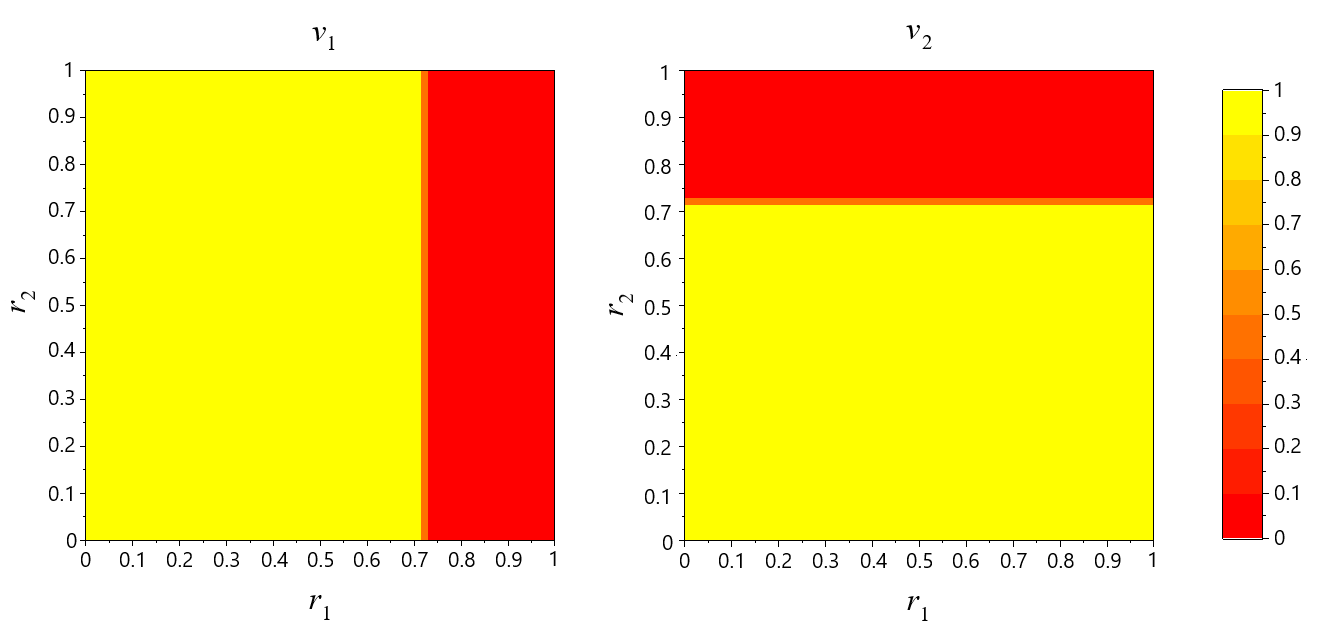
\includegraphics[scale=0.43]{./img/PD-neg-payoff.png}}
    \label{fig:pd-neg-payoff}
\end{figure}

Nos interessa saber se esse comportamento é geral ou uma exceção e, por isso, vamos usar um definição mais geral para o pagamento do dilema do prisioneiro, dada por
\begin{equation}
    \label{payoffGeralPD}
    B=
    \begin{bmatrix}
        R & S\\ 
        T & P 
    \end{bmatrix}
\end{equation}
onde $R$ é a recompensa pela cooperação entre os jogadores, $T$ é a tentação para trair, $P$ é a punição pela traição mútua e $S$ é o pagamento do ingênuo, que foi traído. Para que esses valores representem um dilema do prisioneiro eles devem respeitar a seguinte restrição.

\begin{equation}
    \label{desigualdadePD}
    T>R>P>S
\end{equation}

Assim, a equação de replicação para um dilema do prisioneiro geral é dada por

\begin{equation}
\begin{split}
    \label{eqRepPDGeral}
    \dot{x}_{i,s}&= \!\begin{multlined}[t]
        x_{i,s}(1-x_{i,s})\left\{x_{j,s}\left[r_i(R-T)+(1-r_i)(R-S) \right] \right.\\
        + \left. (1-x_{j,s})\left[r_i(S-P)+(1-r_i)(T-P)\right] \right\}
    \end{multlined} \\
    &= \!\begin{multlined}[t]
    x_{i,s}(1-x_{i,s})\left\{r_i \left[x_{j,s}(R-T)+(1-x_{j,s})(S-P) \right] \right. \\
    + \left. (1-r_i)\left[ x_{j,s}(R-S) + (1-x_{j,s})(T-P)\right] \right\}
    \end{multlined}
\end{split}
\end{equation}

Um jogador não muda sua estratégia quando $\dot{x}_{i,s}=0$. Portanto, vamos assumir que $\dot{x}_{i,s}=0$ para algum perfil de estratégias $\BS{X}$ e, assim, a equação $\eqref{eqRepPDGeral}$ se torna
\begin{equation}
    0 = \!\begin{multlined}[t]
        r_i \left[x_{j,s}(R-T)+(1-x_{j,s})(S-P) \right] \\
    + (1-r_i)\left[ x_{j,s}(R-S) + (1-x_{j,s})(T-P)\right]
    \end{multlined}
\end{equation}
que podemos simplificar da para obtermos
\begin{equation}
    0 = r_i(S-T) + x_{j,s}(R-S) + (1-x_{j,s})(T-P)
\end{equation}
e, por fim, isolamos $r_i$ para obter
\begin{equation}
    \label{rSela}
    r_i=\frac{x_{j,s}(T+S-P-R)+P-T}{S-T}
\end{equation}

Com isso, se a igualdade 
\begin{equation}
    \label{condicaoIndependencia}
    T+S-P-R = 0
\end{equation}
for satisfeita, basta que tenhamos
\begin{equation}
    r_i=\frac{P-T}{S-T}
\end{equation}
para que $\dot{x}_{i,s}=0$ para todo $t>0$, fazendo com que a condição inicial de $i$ seja um hiperequilíbrio. Note que a igualdade $\eqref{condicaoIndependencia}$ é, de fato, satisfeita para os pagamentos de \ref{mpdp}, $R=-2,S=-7,T=0,P=-5$. Além disso, a igualdade $\eqref{rSela}$ nos dá uma forma de encontrar o ponto de sela, onde qualquer variação em $r_i$, para mais ou para menos, vai alterar o resultado do jogo. Também podemos ver uma ligação entre $r_i$ e $x_{j,s}$, que iremos avaliar agora.

Podemos alterar a matriz \ref{mpdp} para que haja uma dependência diretamente proporcional entre $r_i$ e $x_{j,s}$, basta tomar $R=-1$, assim a equação $\eqref{rSela}$ se torna
\begin{equation}
    r_i=\frac{5+x_{j,s}}{7}
\end{equation}

Como $x_{j,s}\in[0,1]$, para valores de $r_i$ no intervalo $[\frac{5}{7},\frac{6}{7}]$ a distribuição de estratégias do jogador $i$ depende diretamente da distribuição de $j$ e, em algumas condições especiais, temos um ponto de equilíbrio interno para cada um desses valores de $r_i$. Discutiremos mais sobre esse ponto de equilíbrio ao final desta seção. Como a matriz de pagamentos é igual para ambos jogadores, esse intervalo de dependência é igual para os dois jogadores e a solução dentro do quadrado $[\frac{5}{7},\frac{6}{7}]\times[\frac{5}{7},\frac{6}{7}]$ dependerá da distribuição de estratégias de ambos. Esse comportamento pode ser observado na figura \ref{fig:pd-neg-payoff-dependant}, onde o ponto de sela da solução se encontra na diagonal do quadrado $[\frac{5}{7},\frac{6}{7}]\times[\frac{5}{7},\frac{6}{7}]$. Também é interessante notar que a estratégia $\textit{silêncio}$ é predominante no nosso gráfico, pois $\textit{delação}$ só é vantajoso para de $r_i$ próximos de $1$.

\begin{figure}[h]
    \caption{Probabilidade do jogador usar \textit{silêncio} ao tomar $R=-1$ no pagamento dado por \ref{mpdp}, onde a condição inicial é 0.5 para todas estratégias para ambos jogadores.}
    \centerline{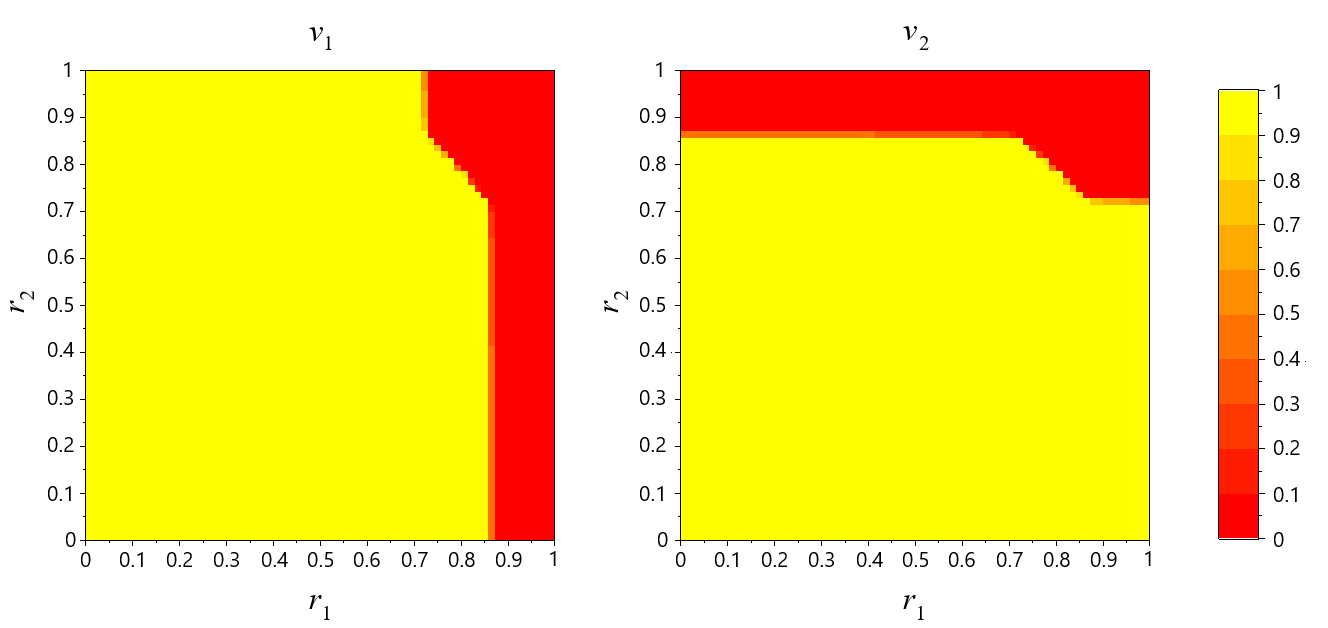
\includegraphics[scale=0.43]{./img/PD-neg-payoff-dependant.png}}
    \label{fig:pd-neg-payoff-dependant}
\end{figure}

Da mesma maneira, podemos novamente usar o pagamento definido em \ref{mpdp} e tomar $S=-6$ para que haja uma dependência inversamente proporcional entre $r_i$ e $x_{j,s}$, assim a equação $\eqref{rSela}$ se torna
\begin{equation}
    \label{eqQuadradoEx}
    r_i=\frac{5-x_{j,s}}{6}
\end{equation}

Agora temos $[\frac{4}{6},\frac{5}{6}]$ como nosso intervalo de dependência que, novamente, é igual para ambos jogadores. Agora o ponto de sela estará na diagonal do quadrado $[\frac{4}{6},\frac{5}{6}]\times[\frac{4}{6},\frac{5}{6}]$ e, apesar de ainda não ser predominante, a faixa na qual $\textit{delação}$ se torna mais vantajosa aumentou consideravelmente.

\begin{figure}[h]
    \caption{Probabilidade do jogador usar \textit{silêncio} ao tomar $S=-6$ no pagamento dado por \ref{mpdp}, onde a condição inicial é 0.5 para todas estratégias para ambos jogadores.}
    \centerline{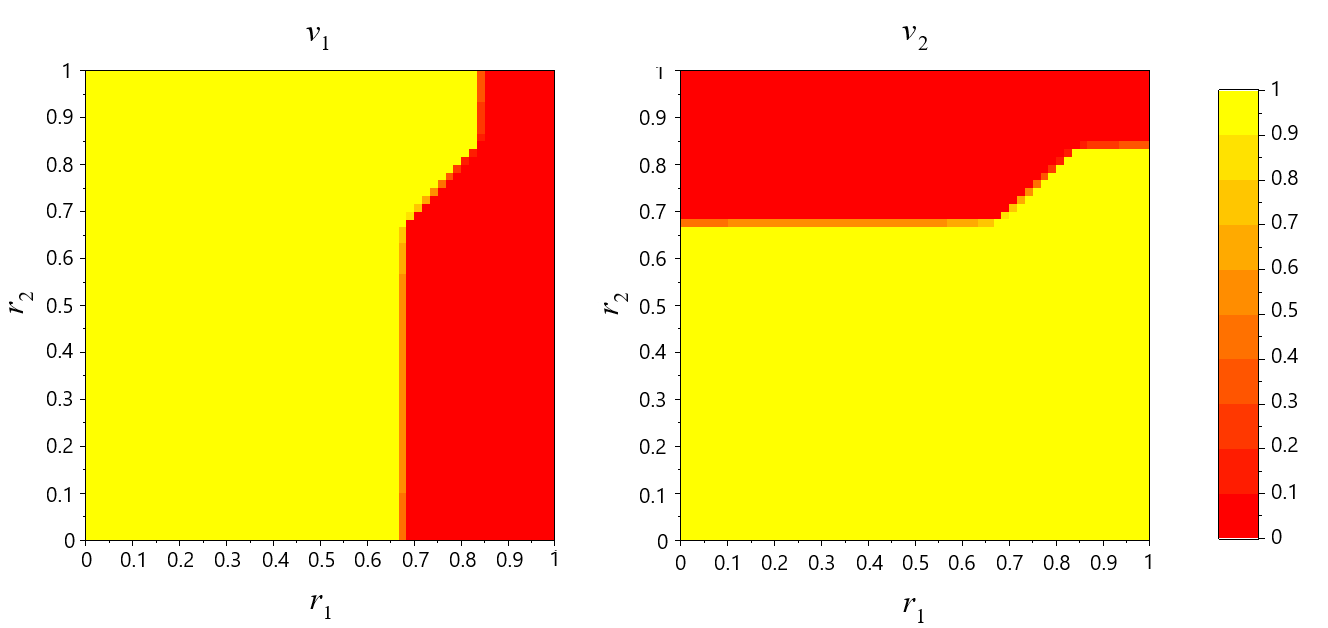
\includegraphics[scale=0.43]{./img/PD-neg-payoff-inverse-dep.png}}
    \label{fig:pd-neg-payoff-inverse-dep}
\end{figure}

A hiper-racionalidade dos jogadores envolvidos faz com que a estratégia $\textit{silêncio}$ se torne, em geral, mais atraente para o jogador mesmo que a condição inicial não esteja muito próxima de $\textit{silêncio}$, enquanto jogadores racionais, mesmo em redes, tendem a preferir $\textit{delação}$ se houver algum vizinho delator \cite{madeo2015}.

Na figura \ref{fig:sobreposicao} temos a sobreposição dos gráficos dos dois jogadores para cada pagamento discutido acima. Assim, podemos ver o resultado do jogo em cada uma das faixas de $r_i$ analisadas anteriormente, explicitando a predominância da estratégia $\textit{silêncio}$ e o fato de que, em muitos casos, um jogador recebe o pagamento do ingênuo $S$, mesmo podendo aumentar seu pagamento efetivo trocando sua estratégia para $\textit{delação}$.

\begin{figure}[h]
    \caption{Sobreposição dos resultados do Dilema do Prisioneiro para cada pagamento apresentado anteriormente. Nos parênteses temos, respectivamente, o resultado do jogador $v_1$ e $v_2$, com $s$ para $\textit{silêncio}$ e $d$ para $\textit{delação}$.}
    \centerline{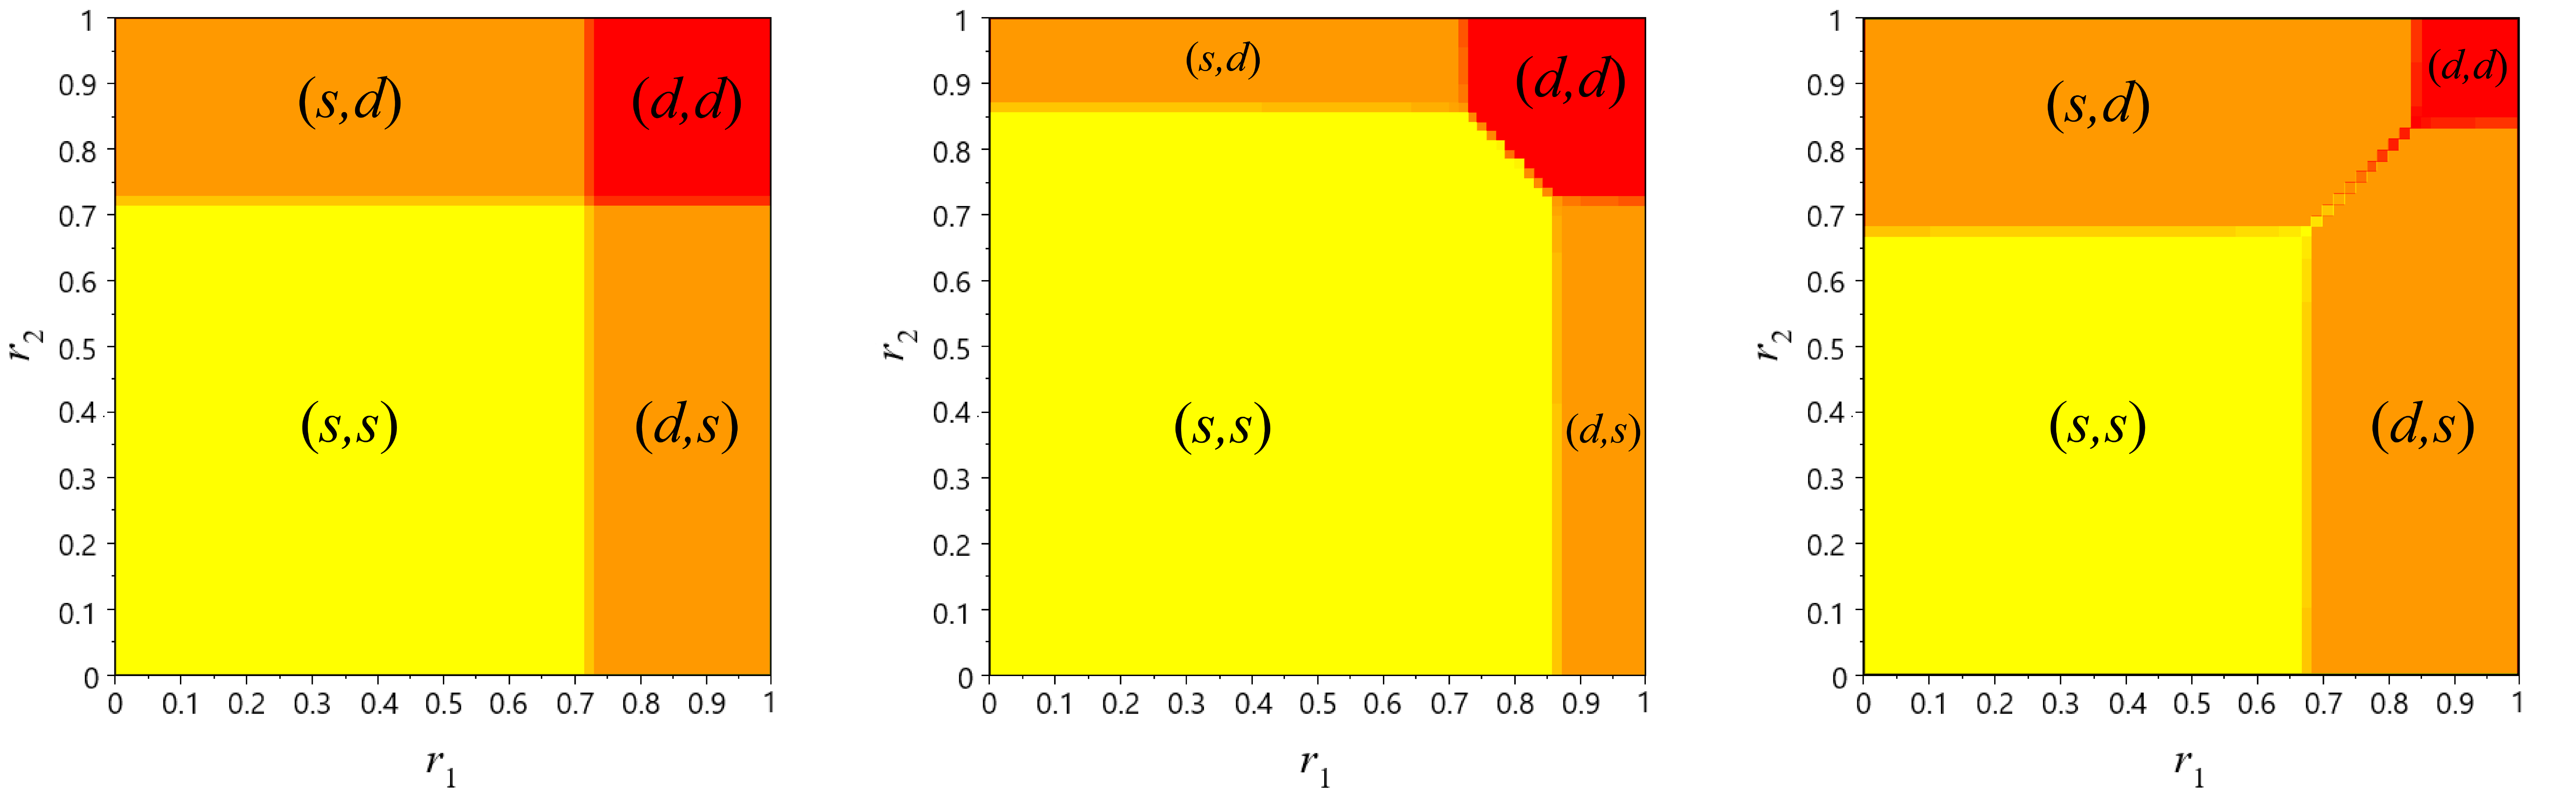
\includegraphics[scale=0.0775]{./img/sobreposicao.png}}
    \label{fig:sobreposicao}
\end{figure}

Essa sobreposição nada mais é do que a soma das probabilidades de $v_1$ e $v_2$ dividida por $2$ exibida na mesma escala das demais figuras desta seção. Assim, as faixas de transição em $\frac{5}{7}$ e nas diagonais dos quadrados $[\frac{5}{7},\frac{6}{7}]\times[\frac{5}{7},\frac{6}{7}]$ e $[\frac{4}{6},\frac{5}{6}]\times[\frac{4}{6},\frac{5}{6}]$ exibem a cor que representa essa média das probabilidades.

Agora iremos analisar a existência dos pontos de equilíbrio interno no interior dos quadrados $[\frac{5}{7},\frac{6}{7}]\times[\frac{5}{7},\frac{6}{7}]$ e $[\frac{4}{6},\frac{5}{6}]\times[\frac{4}{6},\frac{5}{6}]$. Note que podemos reescrever a expressão $\eqref{rSela}$ da seguinte maneira.

\begin{equation}
    x_{j,s}=\frac{r_i(S-T)-P+T}{T+S-P-R}
\end{equation}

Essa expressão nos dá um valor de $x_{j,s}$ em função de $r_i$. Como $j$ não tem conhecimento sobre o valor de $r_i$, esse equilíbrio só existe quando $r_i=r_j$, pois nessas condições teremos a expressão

\begin{equation}
    \label{eqInternoPDHR}
    x_{j,s}=\frac{r_j(S-T)-P+T}{T+S-P-R}
\end{equation}

Assim, para valores de $r_i=r_j$ dentro da zona de transição temos um ponto de equilíbrio instável em $\eqref{eqInternoPDHR}$. Para exemplificar vamos usar o jogo que nos deu a equação $\eqref{eqQuadradoEx}$, onde para valores de $r_i=r_j\in(\frac{4}{6},\frac{5}{6})$ teremos um ponto fixo interno e instável em

\begin{equation}
    \label{ptoEqCela}
    x_{i,s}=5-6r_i=5-6r_j=x_{j,s}
\end{equation}

Os gráficos gerados nesse capítulo não capturaram esses pontos fixos, pois a condição inicial $[0.5,0.5]^T$ não pertence à nenhuma das zonas de transição dadas nos exemplos. Para demonstrar a instabilidade deste ponto, basta considerar a equação de replicação dada por esta matriz de pagamentos, que é a seguinte.

\begin{equation}
    \dot{x}_{i,s}= 5-6r_i - x_{j,s}
\end{equation}

Como o jogo é simétrico, a equação é a mesma para ambos jogadores. Como concluímos acima, se $x_{j,s}=5-6r_i$, temos $\dot{x}_{i,s}=0$, porém qualquer alteração em $x_{j,s}$ fará com que $\dot{x}_{i,s}\neq 0$. Novamente, pela simetria, qualquer perturbação no equilíbrio fará com que o outro jogador também saia do equilíbrio. Então, tomando $r_i=r_j$ e $x_{i,s}=x_{j,s}$ como na relação $\eqref{ptoEqCela}$, dado $\epsilon>0$, $\forall x_{i,s}'\neq x_{i,s}$ tal que $|x_{i,s}'-x_{i,s}|<\epsilon$ teremos que $\dot{x}_{j,s}\neq 0$. Pela simetria do jogo, o mesmo acontece para o jogador $i$. Note que, se $x_{j,s}>5-6r_i$ teremos $\dot{x}_{i,s}<0$, além disso se $x_{j,s}<5-6r_i$, temos $\dot{x}_{j,s}>0$. Com isso, concluímos que o ponto de equilíbrio dado por $\eqref{ptoEqCela}$ é, de fato, instável.

% O jogo dos Colegas de Quarto
\chapter{O jogo dos colegas de quarto}

Vimos que a assimetria de informação pode levar o jogo a um resultado que não é ótimo para nenhum dos jogadores, onde um jogador é capaz de, até mesmo, aumentar seu pagamento ao mudar de estratégia unilateralmente. É de nosso interesse saber se esse também o caso quando jogo se repete ao longo do tempo, sendo regido pela equação $\eqref{defEqRepHR}$, onde esperamos que os jogadores sejam capazes de identificar explorar as hiperpreferências dos demais. Para fazer essa análise, vamos definir o jogo dos colegas de quarto, onde podemos observar como o conflito de interesses e preferências interfere no perfil de estratégias ao longo do tempo. É importante ressaltar que este jogo ainda é como nos jogos clássicos, onde a cada instante dois jogadores vizinhos são selecionados de maneira aleatória para jogar entre si e os jogadores selecionados irão jogar uma estratégia pura com uma dada probabilidade. Dito isso, nós usaremos uma analogia com a rotina de colegas de quarto para que o jogo fique mais fácil de ser interpretado, mesmo que ela possa perder um pouco o seu sentido se pensarmos na forma como ocorrem os encontros entre jogadores em jogos evolucionários.

Neste jogo temos três jogadores em um grafo completo, um triângulo no qual todos interagem entre si, onde os jogadores são colegas de quarto, porém existem sentimentos não correspondidos que mudam a forma como eles interagem. Para ilustrar essa dinâmica vamos considerar duas estratégias, ser $\textit{organizado}$ e ser $\textit{desordeiro}$, ou $O$ e $D$. Consideramos que cada um possui sua própria matriz de pagamentos, definidas abaixo. Lembre-se que a entrada $b_{k,i,j}$ da matriz $B_k$ é o pagamento do jogador $k$ ao usar a estratégia $i$ contra a estratégia $j$, com $k\in\{u,v,w\}$ e $i,j\in\{O,D\}$, neste caso.

\begin{equation}
    \label{payoffLoveTri}
    B_u=
    \begin{bmatrix}
        0 & 1\\ 
        0 & 0 
    \end{bmatrix},
    B_v=
    \begin{bmatrix}
        0 & 0\\ 
        1 & 0 
    \end{bmatrix},
    B_w=
    \begin{bmatrix}
        1 & 0\\ 
        0 & 0 
    \end{bmatrix}
\end{equation}

Note que $u$ e $v$ se complementam, pois $u$ só possui pagamento ao jogar $O$ com alguém que jogue $D$ e $v$ só possui pagamento ao jogar $D$ para alguém que jogue $O$, enquanto $w$ só se beneficia ao jogar $O$ contra $O$. Assim, com jogadores racionais, é esperado que o perfil $(e_1,e_2,e_1)$ seja o resultado final do jogo, onde $u$ e $v$ irão se relacionar de maneira complementar, $v$ receberá um pagamento de ambas suas relações e $w$ irá conseguir algum benefício apenas de sua relação com $u$.

Este jogo se torna interessante ao considerarmos jogadores hiper-racionais, pois as interações entre eles deixam de ser tão óbvias. Considere o caso no qual o jogador $u$ possui sentimentos por $v$, $v$ possui sentimentos por $w$ que, por sua vez, possui somente amor próprio. Essas relações podem ser representadas através da seguinte matriz de preferências.
\begin{equation}
    \label{prefPosLoveTri1}
    \Rc=
    \begin{bmatrix}
        \frac{1}{2} & \frac{1}{2} & 0\\ 
        0 & \frac{3}{5} & \frac{2}{5} \\
        0 & 0 & 1
    \end{bmatrix}
\end{equation}

Assim, as equações de replicação de cada jogador serão como segue.

\begin{equation}
    \label{EqRepLoveTri1}
    \left\{\begin{matrix*}[l]
        \dot{x}_{u,O}=x_{u,O}(1-x_{u,O})\left(\frac{3}{4}x_{v,D}+\frac{1}{4}x_{w,D}\right) \\
        \dot{x}_{v,O}=x_{v,O}(1-x_{v,O})\left(-\frac{3}{10}x_{u,O}-\frac{1}{10}x_{w,O}\right) \\
        \dot{x}_{w,O}=x_{w,O}(1-x_{w,O})\left(\frac{1}{2}x_{u,O}+\frac{1}{2}x_{v,O}\right)
    \end{matrix*}\right.
\end{equation}

Pelas equações, podemos concluir que o resultado será o mesmo do jogo clássico, o perfil de estratégias $(e_1,e_2,e_1)$. Isso pode ser observado na figura \ref{fig:love_tri1.png}.

\begin{figure}[h]
    \caption{Evolução do uso da estratégia $O$ para cada um dos colegas de quarto com $\Rc$ dada em $\eqref{prefPosLoveTri1}$,  $[0.5 \; 0.5]^T$ como condição inicial para todos jogadores e $t\in[0,40]$.}
    \centerline{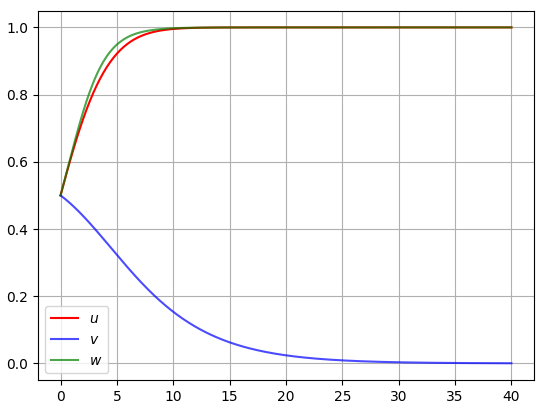
\includegraphics[scale=0.8]{./img/love_tri1.png}}
    \label{fig:love_tri1.png}
\end{figure}

Para tornar o jogo mais interessante vamos supor que a afeição de $v$ por $w$ esteja cada vez maior e, com isso, $v$ passe a valorizá-lo com a mesma intensidade que valoriza a si mesmo. Por conta disso, $u$ começa a desconfiar dos sentimentos de $v$ por $w$ e, por ciúmes, passa a querer o prejuízo de $w$. Essa nova dinâmica pode ser representada pela seguinte matriz de preferências.

\begin{equation}
    \label{prefPosLoveTri2}
    \Rc=
    \begin{bmatrix}
        \frac{2}{5} & \frac{2}{5} & -\frac{1}{5}\\ 
        0 & \frac{1}{2} & \frac{1}{2} \\
        0 & 0 & 1
    \end{bmatrix}
\end{equation}

Com essas mudanças, as equações $\eqref{EqRepLoveTri1}$ serão dadas por
\begin{equation}
    \label{EqRepLoveTri2}
    \left\{\begin{matrix*}[l]
        \dot{x}_{u,O}=x_{u,O}(1-x_{u,O})\left(\frac{2}{5}x_{v,D}+\frac{1}{5}x_{w,D} -\frac{1}{10}x_{w,O}\right) \\
        \dot{x}_{v,O}=x_{v,O}(1-x_{v,O})\left(\frac{1}{4}x_{w,O}-\frac{1}{4}x_{u,O}\right) \\
        \dot{x}_{w,O}=x_{w,O}(1-x_{w,O})\left(\frac{1}{2}x_{u,O}+\frac{1}{2}x_{v,O}\right)
    \end{matrix*}\right.
\end{equation}

Note que a equação de $w$ não mudou e, portanto, se $x_{u,O}>0$ ou $x_{v,O}>0$ teremos que $x_{w,O}\to 1$. Então, assumindo que $x_{w,O}=1$ enquanto $x_{u,O},x_{v,O}\in(0,1)$ para algum $t>0$ , temos que
\begin{equation}
    \label{uDedicav}
    \dot{x}_{u,O}>0 \Longleftrightarrow x_{v,O} \leq \frac{3}{4},
\end{equation}
ou seja, uma condição para que $u$ continue jogando $O$ e agradando ao jogador $v$. Porém, ao mesmo tempo, temos
\begin{equation}
    \label{vDedicau}
    \dot{x}_{v,O} \leq 0 \Longleftrightarrow x_{u,O} \geq x_{w,O},
\end{equation}
que nos dá uma condição para que $v$ não deixe de jogar $D$, que agrada o jogador $u$, para jogar $O$, que agrada o jogador $w$. Caso as condições $\eqref{uDedicav}$ e $\eqref{vDedicau}$ não sejam satisfeitas, teremos como solução o perfil de estratégias $(e_2,e_1,e_1)$, onde $u$ passa a jogar $D$ apenas para diminuir o pagamento de $w$, pois ele não recebe mais nenhum benefício de sua relação com $v$, que agora joga $O$ para aumentar o pagamento de $w$, mesmo não recebendo nenhum pagamento efetivo dessa relação. Essa dinâmica pode ser observada na figura \ref{fig:love_tri2.png}.

\begin{figure}[h]
    \caption{Evolução do uso da estratégia $O$ para cada um dos colegas de quarto com $\Rc$ dada em $\eqref{prefPosLoveTri2}$,  $[0.5 \; 0.5]^T$ como condição inicial para todos jogadores e $t\in[0,120]$.}
    \centerline{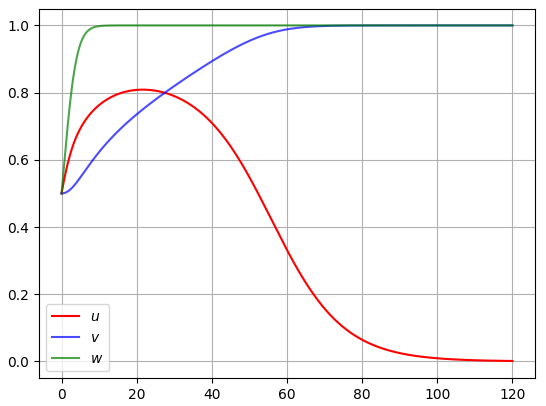
\includegraphics[scale=0.8]{./img/love_tri2.png}}
    \label{fig:love_tri2.png}
\end{figure}

Apesar de parecer simples, essa dinâmica entre colegas de quarto $\textit{organizados}$ e $\textit{desordeiros}$ pode se tornar complicada quando inserimos os sentimentos humanos como variáveis. Neste exemplo conseguimos modelar afeição e ciúmes através das hiperpreferências dos jogadores, exemplificando o que foi dito no capítulo \ref{chap:hiperRacionalidade} e mostrando como a hipótese de racionalidade não é suficiente para modelar o comportamento humano em todas situações.

% Simulações
\chapter{Simulações}

Para que possamos avaliar o efeito que a hiper-racionalidade tem no resultado de um jogos nós iremos simular os mesmos problemas, estruturas e condições iniciais das simulações encontradas em \cite{madeo2015}. A matriz de preferências que usaremos depende do grafo onde a simulação é feita onde as entradas são dadas por
\begin{equation}
    \label{prefComparativo}
    r_{v,u} = \left\{\begin{matrix}
                \frac{1}{2} \text{, se } v=u\\ 
                \frac{1}{2d_v} \text{, se } v\neq u \text{ e } a_{v,u}\neq 0 \\
                 0 \text{, se } a_{v,u}=0
                \end{matrix}\right.,
\end{equation}
onde $d_v$ é o grau do vértice $v$. Em outras palavras, um jogador possui preferência $\frac{1}{2}$ por si e o resto é dividido igualmente entre todos seus vizinhos. As simulações foram feitas para $3$ tipos de grafo estrela em $3$ diferentes condições iniciais para os jogos do dilema do prisioneiro não estrito, biestabilidade e coexistência. As arestas mais grossas na estrela assimétrica ponderada possuem peso $3$, enquanto todas demais arestas possuem peso $1$. 

Vamos começar com o dilema do prisioneiro não estrito, cuja a única diferença do dilema que vimos até o momento é que as desigualdades em $\eqref{desigualdadePD}$ são não estritas. A matriz de pagamentos usada nas simulações é dada por
\begin{equation}
    \label{pagtoPDComparativo}
    B=
    \begin{bmatrix}
        1 & 0\\ 
        \frac{3}{2} & 0 
    \end{bmatrix}
\end{equation}

Podemos ver na figura \ref{fig:prisoner-control.png} o resultado das simulações. Ao contrário do jogo com jogadores racionais, o $\textit{silêncio}$ é predominante dentre os jogadores hiper-racionais e $\textit{delação}$ aparece somente por conta da centralidade de $1$, que distribui o pagamento da tentação para sua vizinhança por conta das hiperpreferências dos jogadores. Porém, ainda temos um equilíbrio misto na estrela assimétrica ponderada para a condição inicial $a$, que surge por conta do incentivo inicial para que $2$ use $\textit{silêncio}$ que é freado quando $1$ passa a usar exclusivamente $\textit{delação}$.

\begin{figure}[h]
    \caption{Probabilidade do jogador usar \textit{silêncio} no dilema do prisioneiro em diferentes grafos estrela com matriz de pagamentos $\eqref{pagtoPDComparativo}$. Na primeira coluna temos a distribuição de estratégias para $t=0$ e nas demais temos a distribuição para $t=100$ nos grafos dados. As simulações para jogadores racionais foram feitas por Madeo e Mocceni e podem ser encontradas em \cite{madeo2015}.}
    \centerline{\includegraphics[scale=0.27]{./img/prisoner-control.png}}
    \label{fig:prisoner-control.png}
\end{figure}

No jogo da biestabilidade um jogador recebe um pagamento somente quando joga contra a mesma estratégia que está usando, onde uma delas pode, ou não, gerar um pagamento maior do que a outra. A matriz de pagamentos que foi usada na simulação é a seguinte.
\begin{equation}
    \label{pagtoBiComparativo}
    B=
    \begin{bmatrix}
        1 & 0\\ 
        0 & 1 
    \end{bmatrix}
\end{equation}

O resultado para as simulações do jogo da biestabilidade pode ser observado na figura \ref{fig:bistability-control.png}. Vemos que, no caso racional, os jogadores sempre querem usar a estratégia que a maioria de sua vizinhança usa, o que leva ao equilíbrio misto na estrela aberta com dissidente central e à dissidência de $2$ e $6$ na estrela assimétrica ponderada com condição inicial $c$. No caso hiper-racional temos uma situação parecida, pois as hiperpreferências acentuam o incentivo por estar na moda, fazendo com que não haja mais o equilíbrio misto na estrela aberta e aumentando a importância das relações de menor peso na estrela assimétrica ponderada.

\begin{figure}[h]
    \caption{Probabilidade do jogador usar a estratégia $1$ no jogo da biestabilidade em diferentes grafos estrela com matriz de pagamentos $\eqref{pagtoBiComparativo}$. Na primeira coluna temos a distribuição de estratégias para $t=0$ e nas demais temos a distribuição para $t=50$ nos grafos dados. As simulações para jogadores racionais foram feitas por Madeo e Mocceni e podem ser encontradas em \cite{madeo2015}.}
    \centerline{\includegraphics[scale=0.27]{./img/bistability-control.png}}
    \label{fig:bistability-control.png}
\end{figure}

No jogo da coexistência um jogador recebe um pagamento somente quando joga contra uma estratégia diferente da que está usando e todos pagamentos são iguais. A matriz de pagamentos que foi usada na simulação é a seguinte.
\begin{equation}
    \label{pagtoCoexComparativo}
    B=
    \begin{bmatrix}
        0 & 1\\ 
        1 & 0 
    \end{bmatrix}
\end{equation}

O resultado para as simulações do jogo da coexistência pode ser observado na figura \ref{fig:coex-control.png}. Ao contrário da biestabilidade, nesse jogo há um incentivo para ser diferente dos seus vizinhos e podemos ver que os resultados em ambos modelos são praticamente iguais, com exceção dos equilíbrios mistos, que são mais próximos da condição inicial no modelo hiper-racional. Isso se deve às hiperpreferências, que diminuem o incentivo para que os jogadores usem uma estratégia diferente da mais usada em sua vizinhança.

\begin{figure}[h]
    \caption{Probabilidade do jogador usar a estratégia $1$ no jogo da coexistência em diferentes grafos estrela com matriz de pagamentos $\eqref{pagtoCoexComparativo}$. Na primeira coluna temos a distribuição de estratégias para $t=0$ e nas demais temos a distribuição para $t=50$ nos grafos dados. As simulações para jogadores racionais foram feitas por Madeo e Mocceni e podem ser encontradas em \cite{madeo2015}.}
    \centerline{\includegraphics[scale=0.27]{./img/coexistance-control.png}}
    \label{fig:coex-control.png}
\end{figure}

Além de possibilitar uma comparação entre jogadores racionais e hiper-racionais, essas simulações mostram como a estrutura do grafo influencia os hiperequilíbrios do jogo. Vimos que, mesmo para jogadores racionais, os vértices mais centrais exercem maior influência no resultado do jogo, uma característica que é acentuada pelas hiperpreferências positivas, que aumentam o impacto da centralidade no pagamento de todos jogadores.


% Conclusão
\chapter{Considerações finais}

A introdução da hiper-racionalidade e da parte social da equação de replicação adiciona mais uma camada de complexidade na dinâmica do replicador e, como vimos, nos permite modelar comportamentos mais complexos. Inicialmente, nós definimos a função de pagamento $\eqref{defPgtoHR}$ para um jogador hiper-racional $v$, que é formada pela soma do pagamento de $v$ com o pagamento dos demais jogadores como percebido por $v$ ponderada pelas hiperpreferências de $v$. Usando esse pagamento, nós definimos o conceito de hiperequilíbrio \ref{defHiperEq}, que é análogo ao equilíbrio de Nash, usando o pagamento para jogadores hiper-racionais, o que facilita a comparação e análise dos resultados para jogadores racionais e hiper-racionais. Vimos a importância dessa separação ao analisar aos efeitos da assimetria de informação em um jogo estático, onde o hiperequilíbrio do jogo, encontrado através da dominância não estrita iterada nos pagamentos virtuais, não é um equilíbrio de Nash, pois um jogador é capaz de melhorar seu pagamento efetivo ao mudar de estratégia unilateralmente, e isso se deve à assimetria de informação do jogo com jogadores hiper-racionais.

Também analisamos o dilema do prisioneiro com jogadores hiper-racionais e mostramos através da expressão $\eqref{rSela}$ para os valores de $r_i$ que o resultado do jogo depende, principalmente, da matriz de pagamentos e das hiperpreferências do jogador. Com isso, mostramos que a cooperação é predominante dentre jogadores hiper-racionais quando consideramos preferências positivas por si e pela vizinhança.

Reescrevemos a equação de replicação usando o pagamento para jogadores hiper-racionais $\eqref{defEqRepHR}$ e demonstramos a existência e unicidade da solução em $\Delta$, a invariância de $\Delta_M$, que hiperequilíbrios e estratégias puras são pontos fixos da equação e que a equação de replicação clássica é um caso especial da equação para jogadores hiper-racionais. Usando a equação $\eqref{defEqRepHR}$ para simular o jogo dos colegas de quarto nós observamos como as hiperpreferências mudam o resultado do jogo, levando um jogador a preferir um pagamento efetivo menor somente para reduzir o pagamento de um adversário. Em seguida fizemos uma comparação entre o modelo introduzido por Madeo e Mocenni \cite{madeo2015} e a equação de replicação hiper-racional, onde vimos que a hiper-racionalidade aumenta a importância das ligações do grafo para as quais o jogador possui alguma preferência, geralmente causando mudanças no estado de equilíbrio do jogo.

A análise do jogo estático termina com a afirmação de que o jogador racional seria capaz de, eventualmente, identificar e explorar o altruísmo de um jogador hiper-racional. Uma oportunidade para um trabalho futuro que temos é a análise desses jogos iterados e, até mesmo, de como as estratégias do torneio de Axelrod se comportam com a inserção de jogadores hiper-racionais. Podem ser feitas competições mistas, com jogadores racionais e hiper-racionais, onde podemos dividir os vencedores em efetivos e virtuais, para o pagamento efetivo e para o pagamento virtual respectivamente, e avaliar se jogadores hiper-racionais se o altruísmo é capaz de aumentar os pagamentos individuais e globais do jogo.

Em 2020 foi publicado em \cite{tilman2020evolutionary} um modelo para jogos evolucionários com feedbacks ambientais, que é uma dinâmica comum em sistemas socioecológicos, evolucionário-ecológicos e psicológico-econômicos. A inserção de jogadores hiper-racionais nesse contexto pode mudar os equilíbrios e ciclos do jogo, provendo uma nova visão sobre o problema.

Além disso, neste trabalho não analisamos a estabilidade das soluções encontradas para jogadores hiper-racionais, nem o efeito da rede nessas soluções. Essa é mais uma oportunidade para trabalhos futuros, junto da análise dos efeitos da hiper-racionalidade em outros jogos e, até mesmo, na aplicabilidade deste modelo em problemas reais nas diversas áreas citadas nas quais a teoria dos jogos possui aplicações.


%
%	Referencias bibliograficas:
%
\bibliographystyle{acm}  % formatacao do estilo das referencias

%	Bibliografia com o sistema nativo:
%
	% \begin{thebibliography}{9}
	% 	\addbibtocontents
	% 	\bibitem{lamport94}
	% 	  Leslie Lamport,
	% 	  \textit{\LaTeX: a document preparation system},
	% 	  Addison Wesley, Massachusetts,
	% 	  2nd edition,
	% 	  1994.
	% \end{thebibliography}

%	Bibliografia com Bibtex:
%
\bibliography{./bib/ref}
%
%	Apendices:
%
%\appendix % formatacao do estilo dos apendices

%	Apendice A - Algoritmos:
%	\chapter{Algoritmos}
%		\lipsum[29]
%		\section{Primeira seção}
%			\lipsum[30-31]
%		\section{Segunda seção}
%			\lipsum[32-33]
%		\section{Terceira seção}
%			\lipsum[34-35]

\end{document}
